\documentclass[spanish,12pt,letterpaper,oneside]{book}
\usepackage[spanish]{babel}
\usepackage[utf8]{inputenc}
\usepackage[left=3cm,top=2.0cm,right=2.4cm,bottom=2.9cm]{geometry}
%\usepackage[pdftex,hyperindex,breaklinks]{hyperref}
\usepackage{hyperref}
\usepackage{tabularx}
\usepackage[pdftex]{graphicx}
\usepackage{amssymb}
\usepackage{amsmath}
\usepackage{mathrsfs}
\usepackage{fancybox}
\usepackage{fancyvrb}
\usepackage{fancyhdr}
\usepackage{tikz}
\usepackage{index}
\usepackage{enumerate}
\usepackage{setspace}
\usepackage{boxedminipage}
\usepackage{listings}
\usepackage{natbib}
\usepackage{url}
\usepackage{lastpage}
\usepackage{color}
\usepackage{xcolor}
\usepackage{float}
\usepackage{multicol}
\usepackage{algorithm}
\usepackage{algorithmic}
\usepackage{slashbox,pict2e}
\usepackage{adjustbox}
\renewcommand{\algorithmicrequire}{\textbf{Input:}}
\renewcommand{\algorithmicensure}{\textbf{Output:}}


\renewcommand{\baselinestretch}{2}

\newenvironment{itemize_estret}{
\begin{itemize}
  \setlength{\itemsep}{1pt}
  \setlength{\parskip}{0pt}
  \setlength{\parsep}{0pt}
}{\end{itemize}}

\newenvironment{enumerate_estret}{
\begin{enumerate}
  \setlength{\itemsep}{1pt}
  \setlength{\parskip}{0pt}
  \setlength{\parsep}{0pt}
}{\end{enumerate}}

\newenvironment{description_estret}{
\begin{description}
  \setlength{\itemsep}{1pt}
  \setlength{\parskip}{0pt}
  \setlength{\parsep}{0pt}
}{\end{description}}


% Colors
\newcommand{\blue}{\textcolor{blue}}
\newcommand{\red}{\textcolor{red}}
\newcommand{\green}{\textcolor{green}}
\newcommand{\oran}{\textcolor{orange}}
\newcommand{\gray}{\textcolor{gray}}
\definecolor{gray97}{gray}{.97}
\definecolor{gray75}{gray}{.75}
\definecolor{gray45}{gray}{.45}

\lstset{
     frame=single,
     framerule=0pt,
     aboveskip=0.5cm,
     framextopmargin=3pt,
     framexbottommargin=3pt,
     framexleftmargin=0.4cm,
     framesep=0pt,
     rulesep=.4pt,
     backgroundcolor=\color{gray97},
     rulesepcolor=\color{black},
     language=C,
     showstringspaces = false,
     basicstyle=\scriptsize\ttfamily,
     keywordstyle=\bfseries\color{green!70!black},
     commentstyle=\itshape\color{purple},
     %identifierstyle=\color{red},
     stringstyle=\color{orange},
     %commentstyle=\color{gray45},
     %keywordstyle=\bfseries,
     numbers=left,
     numbersep=13pt,
     numberstyle=\scriptsize,
     numberfirstline = false,
     breaklines=true,
     emph = {[1]\_\_device\_\_, \_\_global\_\_, \_\_syncthreads,
             pragma, omp, parallel, private, threadIdx, blockDim, blockIdx,
             cudaThreadSynchronize, while, total, main,dim3},
     emphstyle={[1]\color{blue!70!black}},
   }

% minimizar fragmentado de listados
\lstnewenvironment{listing}[1][]{\lstset{#1}\pagebreak[0]}{\pagebreak[0]}

\lstdefinestyle{consola}{basicstyle=\scriptsize\bf\ttfamily,
                         backgroundcolor=\color{gray75},
                        }

\pagestyle{fancy}

\rhead[]{\leftmark}
\lhead[\rightmark]{}
\lfoot[\thepage]{Left Foot}
\rfoot[Right Foot]{\thepage}
\cfoot{}

%\renewcommand{\listalgorithmname}{Algorithms index}
\renewcommand{\chaptermark}[1]{\markleft{\thechapter #1}}
\renewcommand{\sectionmark}[1]{\markright{\thesection #1}}
\renewcommand{\chaptermark}[1]{\markboth{\chaptername \ \thechapter. #1}{}}

\newcommand{\contrib}[3]{#1\quad$<$\texttt{#2}$>$%
{\small\\\quad\textit{#3}}\\[1ex]}

\newcommand{\titulo}{%
    High Frequency Trading and Graphics Processing Unit.
}%
\newcommand{\autor}{Jonathan Andrés Antognini Cavieres}

\title{\titulo}
\author{\autor}

\date{TBD, 2014}
\frenchspacing
\makeindex


\begin{document}
    %\frontmatter
\thispagestyle{empty}

\begin{center}

{\large\sc Universidad Técnica Federico Santa María}\\
{\large\sc Departamento de Informática}

\vspace{5mm}


\includegraphics[width=0.4\textwidth]{images/utfsm}
\end{center}

\vspace*{\stretch{3}}

\begin{center}
    \begin{LARGE}
        \textbf{\titulo}
    \end{LARGE}
\end{center}

\vspace*{\stretch{5}}

\begin{center}
{\large por}\\
{\huge \autor}
\end{center}


\vspace*{\stretch{5}}

\begin{center}
{\large Tesis para optar al título y grado de}\\
\vspace*{10mm}
{\Large Ingeniero Civil en Informática}\\
\end{center}

\vspace*{\stretch{5}}


\begin{center}
{\large Valparaiso, Chile}\\
{\large TBD, 2013}\\[2mm]
\end{center}

\vspace*{\stretch{1}}

\pagebreak

\thispagestyle{empty}

\begin{center}
{\Large Universidad Técnica Federico Santa María} \\
{\Large Departamento de Informática}\\
{\Large Valparaiso - Chile}\\
\end{center}

\vspace*{\stretch{1}}

\begin{center}
{\large TITULO DE LA MEMORIA:}\\
{\large \textbf{\titulo}}
\end{center}

\vspace*{\stretch{1}}

\begin{center}
{\large AUTOR:}\\
{\large \textbf{\autor}}\\
\end{center}

\vspace*{\stretch{2}}

{\large TRABAJO DE GRADO, presentado en cumplimiento parcial de los requisitos
para el título de Ingeniero Civil en Informática de la Universidad Técnica
Federico Santa María.}

\vspace*{\stretch{5}}
\pagestyle{empty}

\begin{table}[ptbh]
    \begin{tabular}[c]{lc}
    {\large Prof. Dr. Luis Salinas, UTFSM}   & \line(1,0){200}  \\
                                             & {\large Profesor Guía } \\
                                             & \\
                                             & \\
    {\large Prof. Dr. TBD TBD, UTFSM}        & \line(1,0){200}  \\
                                             & {\large Correferente } \\
                                             & \\
                                             & \\
    \end{tabular}
\end{table}

\vspace*{\stretch{1}}

\begin{center}
{\large Valparaiso, Chile}\\
{\large TBD, 2013}\\[2mm]
\end{center}



    \begin{spacing}{.97}
        \newpage
        \vspace*{5cm}
\pagestyle{empty}
\begin{quotation}
\begin{itshape}
ASD
\vspace{2cm}

ASD
\vspace{2cm}

ASD
\end{itshape}
\end{quotation}


        \newpage
    	%TODO
        %\begin{spacing}{.97}
\vspace*{2cm}
\thispagestyle{empty}
%\begin{center}
{\bfseries \Huge Abstract }
\vspace{1.5cm}

\begin{quotation}
The technical analysis of stock markets and foreign exchange market has been
used in order to forecast the behavior of the prices of a certain stock
or currency. Such analysis is based on the detection patterns of
a financial time series, which are known by its non-stationary and random
behavior.

%El análisis técnico de los mercados bursátiles y de divisas se ha utilizado
%para intentar predecir el comportamiento futuro de los precios de un activo o
%una divisa. Dicho análsis se basa en la detección de patrones en una serie
%temporal financiera, las que son conocidas por su comportamiento no
%estacionario y comportamiento aleatorio. 

An interest pattern to address is the integration and cointegration between the
prices of certain stocks or currencies, which establish that when two or more
time series are cointegrated, and considering that both processes are
non-stationary, such as as financial time series, there is a long term
equilibrium relation which link both series such that the relation is
stationary.  The model that take advantage of this scenario is the Vector Error
Correction (VECM)

%Un patrón de interés de estudio es la integración y cointegración entre los
%precios de ciertas divisas. Cuando dos o más series de tiempo están
%cointegradas, a pesar de que ambos procesos no sean estacionarios, como es el
%caso de las series de tiempo financieras, existe una relación de equilibrio a
%largo plazo que vincula ambas series tal que esta relación sea estacionaria. El
%modelo que permite aprovechar este partón es el Vector Error Correction Model
%(VECM).

The cointegration of pairs of currencies have been modeled in several studies,
particularly with FOREX data, which through software tools such as Matlab,
Eviews, etc.  it is possible to computationally forecast the behavior of those
time series.

%Existen varios trabajos donde modelan este problema con pares de monedas,
%particularmente con las series de tiempo del Foreign Exchange Market (FOREX).
%Además mediante herramientas computacionales como matlab, eviews, etc. es
%posible predecir computacionalmente el comportamiento de dichas series de
%tiempo.

However, an important aspect of this kind of series are their online nature,
since every second more information is generated due the Ask or Bid prices,
topic which hasn't been addressed completely.  VECM is a matricial model which,
if it is used in an online context, matrix updates are required to forecast.
%which implies the solution of a matricial system equation, to be able to
%forecast.

%Sin embargo un foco importante de este tipo de series es su caracter
%\emph{Online}, ya que a cada segundo se genera nueva información en el sistema
%debido a la compra o venta de divisas. Tema que no ha sido abordado
%completamente en la literatura. VECM es un modelo matricial, que desde el punto
%de vista \emph{Online}, sufre ciertas actualizaciones de valores, y para poder
%predecir es necesario resolver un sistema matricial.

On this work, we present the VEC, Sliding Windows VEC and Online VEC Models.
The objective of the Online VECM is to optimize the computational calculations,
reducing the number of times that the cointegration vectors are calculated.
Additionally, a class diagram and their implementation associated to Use Cases
was developed, considering: data reading, data re-sample in certain frequency,
graphics, metrics, etc. Additionally, we developed a couple of CUDA routines,
in order to optimize the calculation.

%En este trabajo se presenta el modelo VEC, el modelo VEC para ventanas
%deslizantes y la implementación \emph{Online} que busca optimizar cálculos
%computacionales reduciendo la cantidad de veces que se calculan los vectores de
%cointegración. Para ello se creo un diagrama de clases asociado a los casos de
%uso del modelo, considerando entre ello: lectura de datos, resample a cierta
%frecuencia, gráficos de resultados, etc.

I present the result of a set of tests with different currencies, ensuring all
the conditions to apply this model. The results shows that the Online VEC Model
version, reduce almost 50\% the execution time, maintaining the algorithm
accuracy. 

%Se realizaron pruebas con diferentes monedas de FOREX asegurando las
%condiciones para poder aplicar el modelo. Los resultados muestran que la
%versión \emph{Online} del modelo VEC, disminuye cerca del 50\% el tiempo de
%ejecución sin comprometer la precisión del algoritmo. Además se implementaron
%rutinas en CUDA para optimizar los tiempos de ejecución.

{\bf Keywords:} VECM, VAR, FOREX, GPU.
\end{quotation}

\newpage
% Español

\vspace*{2cm}
\thispagestyle{empty}
%\begin{center}
{\bfseries \Huge Resumen }
\vspace{1.5cm}

\begin{quotation}
El análisis técnico de los mercados bursátiles y de divisas ha sido utilizado
para intentar predecir el comportamiento de los precios de un activo o una
divisa. Dicho análsis se basa en la detección de patrones en una serie temporal
financiera, las que son conocidas por su comportamiento no estacionario y
aleatorio. 


Un patrón de interés de estudio es la integración y cointegración entre los
precios de ciertas divisas, el cual establece que cuando dos o más series de
tiempo están cointegradas, y considerando que ambos procesos no sean
estacionarios (como es el caso de las series de tiempo financieras), existe una
relación de equilibrio a largo plazo, que vincula ambas series para que esta
relación sea estacionaria. El modelo que permite aprovechar este partón es el
Vector Error Correction Model (VECM).

Existen varios trabajos donde modelan este problema con pares de monedas,
particularmente con las series de tiempo del Foreign Exchange Market (FOREX),
las cuales mediante herramientas computacionales como Matlab, Eviews, entre
otros, es posible predecir computacionalmente el comportamiento de dichas
series de tiempo.

Sin embargo un foco importante de este tipo de series es su carácter
\emph{Online}, ya que a cada segundo se genera nueva información en el sistema
debido a la compra o venta de divisas, el cual no ha sido abordado
completamente en la literatura.  VECM es un modelo matricial, que desde el
punto de vista \emph{Online}, sufre ciertas actualizaciones de valores, lo que
implica que para poder realizar una predicción es necesario resolver un sistema
matricial.

En este trabajo se presenta el modelo VEC, el modelo VEC para ventanas
deslizantes y la implementación \emph{Online} que busca optimizar cálculos
computacionales, reduciendo la cantidad de cálculo de los vectores de
cointegración.  Complementariamente, se creó un diagrama de clases asociado a
los casos de uso del modelo, considerando entre ello: lectura de datos,
resampleo a cierta frecuencia, gráficos de resultados, etc.

Se realizaron pruebas con diferentes monedas de FOREX, asegurando las
condiciones necesarias para poder aplicar el modelo. Los resultados muestran
que la versión \emph{Online} del modelo VEC, disminuye cerca del 50\% el tiempo
de ejecución sin comprometer la precisión del algoritmo. Adicionalmente, se
implementaron rutinas utilizando CUDA para optimizar el cálculo.

{\bf Palabras claves:} VECM, VAR, FOREX, GPU.

\end{quotation}

        \addcontentsline{toc}{section}{\contentsname}
\tableofcontents
%\addcontentsline{toc}{subsection}{\listalgorithmname}
%\listofalgorithms
\addcontentsline{toc}{subsection}{\listfigurename}
\listoffigures
\addcontentsline{toc}{subsection}{\listtablename}
\listoftables


        \pagestyle{fancy} 
        \chapter{Introducción}
        \label{ch:introduction}
        \parindent=1.5em

A través de los años el hombre ha presentado un cambio sustancial en su nivel de vida; los conocimientos que ha logrado acumular y aplicar han sido para su beneficio,
y han cambiado radicalmente su modo de vivir. Existe una notable diferencia entre el hombre de hace unas cuantas décadas y el hombre moderno. Tal diferencia se ha
dado por el desarrollo de la ciencia, que está estrechamente relacionada con la innovación tecnológica. Por esta razón se amplía el contenido de cómo ha
evolucionado la ciencia y la tecnología en el mundo, su origen remoto, los países que más han aportado en esta área y su respectiva utilización, ya sea para
el desarrollo o la destrucción. Como se sabe, la tecnología se está haciendo presente en todas y cada una de las áreas de investigación, como física, química, 
biología, computación, y lo que es de interés para este documento es el área de los mercados financieros \cite{watsham1997quantitative}.

Esta memoria está enfocada a abordar un problema relacionado con las series financieras de alta frecuencia y una forma particular de poder realizar pronósticos tomando 
en cuenta las distintas características de naturaleza propia de este tipo de datos. Se pretende abordar esta problemática con metodologías computacionales, 
aplicando algunos análisis matemáticos útiles para esta área. El problema es de carácter financiero, por lo que es necesario contextualizar el tema mediante 
conceptos, criterios y términos generales asociados al área.

Este capítulo tiene como objetivo introducir los conceptos de series de tiempo financieras, sus orígenes y la alta frecuencia.

\section{Mercados Financieros}

El mercado financiero es un espacio con marco institucional que permite poner en contacto a oferentes y demandantes para que efectúen
transacciones financieras. La idea de mercado como foro organizado a la que acuden agentes económicos para efectuar transacciones
queda reducida en el mundo financiero como las bolsas de valores \cite{mishkin2006financial}.

El concepto de mercado financiero se utiliza en general para referirse a cualquier mercado organizado en el que se negocien instrumentos financieros
de todo tipo, como acciones, divisas, etc. El espacio para generar estas interacciones no necesariamente debe ser físico. Por otro lado, el negociar
instrumentos financieros implica a grandes rasgos: definir su precio e intercambiarlos, por ende, estos mercados están basados en
las fuerzas de oferta y demanda, ubicando a todos los oferentes en el mismo lugar, y así facilitarle la búsqueda a los demandantes. Dentro
de este tipo de mercado se distinguieron bloques de estudio en la economía moderna \cite{jensen1984theory}.

Una de las razones que hace importante este tipo de mercado, es su funcionalidad, ya que permiten: por un lado aumentar el capital, siendo esto uno 
de los casos favorables, ya que también hay probabilidades considerables de disminuir el capital; comercio internacional, como en los mercados de 
divisas, por ejemplo Forex; y reunir a quienes necesitan recursos financieros, con los que tienen recursos financieros. Factores que permiten generar los 
efectos de oferta y demanda.

En este tipo de mercado se definen los siguientes términos \cite{nevmyvaka2003electronic}:
\begin{itemize}
	\item \emph{Dealer}: Un dealer es un ente presente en los mercados que está dispuestos a comprar o vender.
	\item \emph{Orders}: Operación de compra/venta de activos.
	\item \emph{Bid price}: Precio al cual un \emph{dealer} está dispuesto a comprar.
	\item \emph{Ask price}: Precio al cual un \emph{dealer} está dispuesto a vender.
	\item \emph{Market orders}: instrucción del cliente al dealer, de comprar o vender al mejor precio posible dentro de los valores actuales del mercado.
		Esto asegura la realización de la transacción, pero no el precio.
	\item \emph{Limit orders}: es una orden para comprar a un valor máximo (precio determinado), o para vender a un valor mínimo (precio determinado).
		Esto le da al cliente el control sobre el precio al que se ejecuta el comercio, sin embargo, no garantiza la realización de la transacción.
\end{itemize}

El conjunto de \emph{Limit orders} forman los \emph{books} para cierto instrumento, los cuales proveen información detallada del mismo. Con estos datos
se forman los llamados bid-ask spreads, que es la diferencia entre el precios cotizados para una venta inmediata (oferta) y una compra inmediata (bid). 
También se generan los bid-ask qoute, el cual define cotas para el precio de transacción.

\subsection{Mercados bursátiles}
Los mercados bursátiles están clasificados dentro de los mercados de capitales, en donde se negocian activos financieros. Este tipo de mercado provee financiamiento
por medio de la emisión de acciones y permiten luego el intercambio de estas. La aplicación más directa de este tipo de mercados, son las bolsas de valores, cuyo
origen se remonta a finales del siglo XV en las ferias medievales de Europa. Las bolsas de valores se pueden definir como mercados organizados y especializados, en 
los que se pueden realizar transacciones de títulos de valores por medio de intermediarios autorizados. Estas bolsas ofrecen al público y a sus miembros facilidades, 
mecanismos e instrumentos técnicos que facilitan la negociación de títulos de valores susceptibles de ofertas públicas, y precios determinados mediante subasta \cite{levine1998stock}.

La principal función de las Bolsas de Valores es proporcionar a los participantes información objetiva, completa y permanente de los valores
y las empresas inscritas en la bolsa, sus emisiones y las operaciones que en ella se realicen. Además debeb supervisar las actividades. Las componentes de este 
sistema son los activos y las instituciones financieras, cuya misión es contactar demandantes y oferentes en los mercados donde se negocian los diferentes instrumentos 
o activos financieros. En el documento se hablará de instrumento, ya que pueden ser acciones, divisas, etc. los cuales quedan generalizados bajo ese concepto.

Dentro de los estudios de la economía, se habla de que este tipo de mercado es de competencia perfecta, ya que posee características
como: elevado número de compradores y vendedores; La decisión individual de cada uno de ellos ejercerá escasa influencia sobre el mercado global; 
Homogeneidad de los productos, es decir, no existen diferencias entre productos que venden los oferentes; Transparencia del mercado, todos los 
participantes tienen pleno conocimiento de las condiciones generales en que opera el mercado; Libertad de entrada y salida de empresas, todos 
los participantes, cuando lo deseen, podrán entrar o salir del mercado a costos nulos o casi nulos \cite{mankiw2011principles}. 

Sin embargo, Eugene Fama propuso la Hipótesis de eficiencia de los mercados \cite{malkiel2012efficient}, la cual dice que los mercados son eficientes cuando
son capaces de trasladar a los precios de los instrumentos financieros, todos los datos relevantes, por lo tanto, el precio refleja \emph{toda} la 
información disponible, y lo hace de manera insesgada. Cuando se cumplen estas condiciones, el precio del instrumento financiero se comporta como un 
\emph{Random Walk} \cite{fama1965random}, por lo que los resultados no pueden ser predichos sistemáticamente.

%Sin embargo, han existido varios estudios asociados a la Hipótesis del Mercado Eficiente, la cual dice que cuando los mercados financieros son eficientes, 
%son capaces de trasladar a los precios de los activos, en cualquier momento, todos los datos relevantes de esos activos, es decir, que el precio de esos activos 
%refleja en todo momento toda la información disponible sobre todos los valores y lo hace de manera insesgada. Este término lo propuso Eugene Fama en el año
%1970, para y se refirió a los procesos aleatorios que se comportan como juegos justos, cuyos resultados no pueden ser predichos sistemáticamente.

\section{Series de tiempo financiera}

La mayoría de los fenómenos que se estudian temporalmente, deben tomar en cuenta la dinámica de los proceso con la finalidad tener una 
comprensión general del proceso. Una herramienta útil en dicho objetivo es el análisis de series de tiempo. Una serie de tiempo, es una secuencia de datos, 
medidos en determinado momento de tiempo y ordenados cronológicamente, con esto se genera una secuencia de datos indexados por su marca temporal. Se pueden presentar 
casos de series de tiempo en una multitud de disciplinas como ingeniería, sociología, economía, finanzas por solo mencionar algunas de ellas.

El propósito fundamental es mostrar las técnicas que permitan hacer inferencias del proceso en estudio incluyendo su predicción. Esto se logra estableciendo modelos
probabilísticos hipotéticos que representen a los datos; y en consecuencia, se lleva a cabo el proceso de ajuste, que incluye desde la estimación hasta la 
predicción, una vez que se ha determinado un modelo satisfactorio para la muestra de datos. Los modelos de series deben considerar la naturaleza del fenómeno y 
determinar los factores que pueden ser incluidos en el.

En particular, el análsis de una serie de tiempo financiera puede enfocarse en estudiar de forma teórica y práctica la valoración de cierto instrumento en el tiempo,
como también los volúmenes transados, etc. Lo que se intenta es modelar la incertidumbre generada por las características propias de este fenómeno \cite{tsay2005analysis}. 

%En particular, el análisis de una series de tiempo financiera se refiere a la teoría y práctica de la valoración de instrumentos en el tiempo, 
%intentando modelar la incertidumbre generada por las características propias del fenómeno. Tanto la teoría económica 
%y sus series temporales contienen un elemento de incertidumbre \cite{tsay2005analysis}. 

Las características diferenciadoras han propiciado numerosos trabajos en las áreas de econometría y economía financiera desde los años 60. Por ello, en el área 
financiera las evidencias sobre patrones ha conducido a la formulación de distintos modelos matemáticos.
%financiera las evidencias sobre estructuras ha conducido a la formulación de distintos modelos matemáticos que se estudiarán en esta memoria.

\subsection{Descripción de serie financiera}

Una tendencia en el estudio de las series financieras, es el estudio del precio de un instrumento en el tiempo.
%Las series de tiempo financieras, se basan en el estudio del precio de un instrumento financiero en el tiempo. 
Existen varios tipos de precios que se pueden analizar, por un lado están los indicadores que se utilizaron en los primeros estudios formales, los cuales 
mostraban información al respecto de los precios de: \emph{apertura}, \emph{cierre}, \emph{el más bajo}, \emph{el más alto}, \emph{promedio}. Esos datos 
estaban orientados a tomar métricas respecto a la frecuencia \emph{día}. Una muestra gráfica de esta información sería la siguiente:
%con estos datos quedaban gráficos como el siguiente:

\begin{center}
	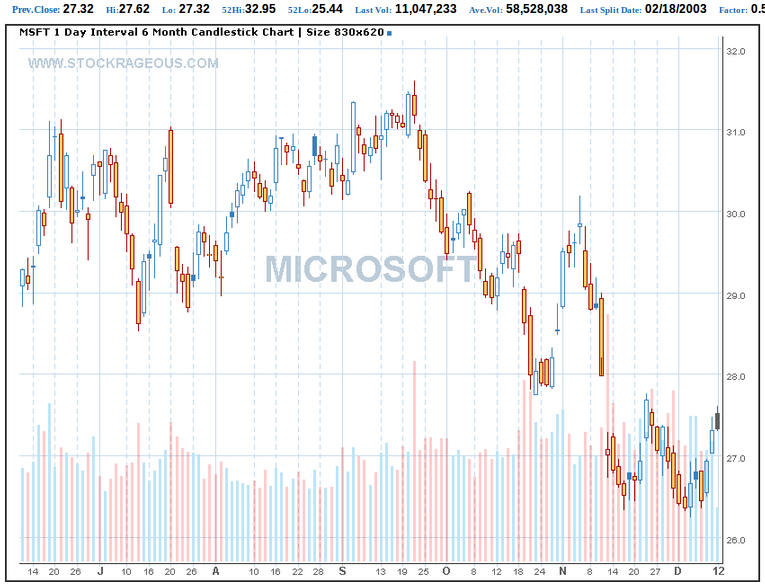
\includegraphics[width=0.8\textwidth]{images/microsoft} \\
	\textbf{Figura 1.} Información de los precios de microsoft en la bolsa. Tomada desde \url{http://www.stockrageous.com/}.
\end{center}

%Esos precios son a nivel diario, ya que los estudios en esos tiempos estaban orientados a esa frecuencia, como los flujos de caja, o análisis gráficos.
Por el tipo de frecuencia considerada en los datos, los estudios realizados estaban orientados a flujos de cajas o análisis gráficos. Sin embargo la data estudiada 
actualmente corresponde a data \emph{intra diaria}, la cual reside en los valores específicos en que se compró o vendió algún instrumento. 
Ese precio se conoce como el \emph{last price}, y corresponde al valor específico con el cual se realizó la transacción. La forma de como se efecúa este evento es 
mediante los \emph{market} o \emph{limit orders}, donde existe una cola de compras o ventas obtenidas mediante los \emph{limit orders} y que cuando se cumpla la 
condición asociada (de vender o comprar a cierto precio), se realiza la transacción y se registra dicho \emph{last price}; 
por otro lado, si se entra a comprar/vender directamente mediante una \emph{market order} también se registra dicho valor. Recopilando esa información, 
se puede generar una secuencia temporal de los \emph{last prices}. Estudios prácticos de estas series generalizan su gráfica con forma de \emph{U},
\cite{biais2012empirical}. 

%Por lo tanto, tomando en cuenta la alta frecuencia de estos datos, se torna muy complicado manejarlo de forma humana, es por esta 
%razón que es necesario realizar análisis cuantitativos usando computadores.

A través de la historia, estas interacciones se realizaban personalmente en las bolsas de comercio, en los llamados \emph{floor market} \cite{jain2005financial},
sin embargo con el avance de las tecnologías, se han implementado distintas plataformas de \emph{trading electrónico}: un método de negociación de instrumentos 
financieros por medios electrónicos \cite{weston2002electronic}. Estas tecnologías se utilizan para reunir a compradores y vendedores a través de plataformas de comercio 
electrónico, como por ejemplo: National Association of Securities Dealers Automated Quotation (NASDAQ), New York Stock Exchange (NYSE), etc. Tomando en cuenta las nuevas 
frecuencias de aparición de datos, en el orden de fracción de segundos, se torna difícil manejar los datos de forma humana, es por esta razón que es necesario realizar análisis 
cuantitativos mediante algoritmos computacionales.

Las series financieras de alta frecuencia tienen características singulares en relación a otras series, como son: 
\begin{itemize}
	\item Frecuencia: la frecuencia en la observación de los datos es mayor que en otro tipo de series de tiempo.
	\item Heterocedasticidad: ocurre cuando la varianza de las perturbaciones no es constante a lo largo de las observaciones.
		Este factor hace inadecuados los modelos desarrollados para series estacionarias.
	\item No estacionalidad: en muchos casos la media y varianza se presentan como no estacionarias.
	\item Información oculta: se pueden encontrar distintos tipos de patrones a diferentes niveles de escala.
\end{itemize}

\subsection{High frequency trading}

Con el paso del tiempo y la implementación de distintos sistemas de trading electrónico, la frecuencia de la data aumentó, pasando de minutos a fracciones de segundos. 
En estos sistemas se define un \emph{Tick}, como unidad atómica de información, particularmente sobre un instrumento determinado.
Esta unidad especifica una gran cantidad de parámetros como la marca temporal, precio, cantidad transada, etc. Los datos de alta frecuencia son un conjunto de datos 
de reportes detallados sobre la actividad y movimiento efectuados sobre un instrumento. Se reúne la información de los ticks con cierto intervalo de tiempo, 
el cual para este tipo de series es variable. El término utilizado para definir este fenómeno no es único \cite{ei2007quantitative}, existen distintos términos
para referirse a este tipo de datos, como (ultra-)high-frequency data, microstructure data, entre otros. 
%\emph{Wei Sun}, señala en \cite{ei2007quantitative} que en la literatura acuñan distintos términos para referirse a este tipo de datos.

Los sistemas informáticos que realizan la labor de facilitar el comercio de instrumentos financieros, son los llamados \emph{Electronic communication networks} (ECN).
Se crearon en 1998, año que fueron autorizados por la \emph{Securities and Exchange Commission}. La SEC es una organización estadounidense creada en 1933 \cite{hasbrouck2004economic}, 
y tiene la responsabilidad de velar por el cumplimiento de las leyes federales las bolsas de valores. Un caso emblemático, fue el 6 de mayo del 2010, fecha en la cual ocurrió el 
\emph{Flash-Crash} \cite{arndt2011high}, dio a lugar a una quiebra financiera estadounidense en el que el índice Dow Jones Industrial Average se desplomó un 9\%.

\section{High Performance Computing}

La capacidad de cómputo de los procesadores actuales ha incrementado, al igual que la cantidad de procesadores de las CPU y también las que tienen las tarjetas de video. Además, la
naturaleza de los problemas que se están estudiando, como simulación de tsunami, series de tiempo financiera, etc. generan una gran cantidad de cómputo, por lo que es
necesario optimizar y hacer más eficientes los algoritmos. Es por esto que nace el concepto de HPC, que es el área de desarrollo que aplica computadores de alto rendimiento 
(clusters) a tareas que implican alta cantidad de cómputo o requieren manejo de grandes volúmenes de información. 
%La idea base consiste en dividir los problemas en sub-problemas que se asignan a diferentes cores de un nodo o diferentes nodos de cálculo, coordinados por un nodo maestro mediante una red de alta velocidad. 

\subsection{Graphics Processing Unit}
%CUDA
Las siglas GPU provienen de Graphics Processing Unit, o en español Unidad de procesamiento gráfico. Para efectos de hardware, la GPU funciona como coprocesador,
pudiéndose utilizar de forma simultánea a la CPU y así aprovechar el potencial que puedan ofrecer ambas al mismo tiempo. Una GPU es un procesador
diseñado para llevar a cabo cálculos necesarios implicados en la generación de gráficos, ya sea, para un video juego, o como para una aplicación que utilice
gráficos en 2D, o 3D. Hoy en día las GPU son muy potentes y pueden incluso superar frecuencias de reloj de una CPU antigua.

Una GPU está formada por cientos de pequeños núcleos que trabajan juntos para procesar los datos de alguna aplicación. Esta arquitectura de procesamiento paralelo
masivo es la que proporciona al GPU su alta capacidad de cálculo. Existen numerosas aplicaciones aceleradas en la GPU que brindan una forma rápida de acceder
a la computación de alto desempeño (High Performance Computing). Durante los últimos años se han desarrollado nuevas tecnologías y arquitecturas
que permiten sacar mayor provecho a sus capacidades \cite{owens2007gpu}.

El concepto implícito en todo este tema es el paralelismo, que es una forma de computación en la cual varios cálculos pueden realizarse simultáneamente,
siempre y cuando no existan dependencias secuenciales entre ellos. Basándose en "divide y vencerás", principio que busca dividir los problemas grandes, para
obtener varios problemas pequeños, que son posteriormente solucionados en paralelo.

La evolución de las tarjetas gráficas ha venido acompañado de un gran crecimiento en el mundo de los videojuegos y las aplicaciones 3D, realizándose grandes
producciones de chips gráficos por parte de grandes fabricantes, como NVIDIA, AMD (ex ATI). Los recientes desarrollos sobre GPU abarcan distintas áreas de la ciencia \cite{kirk2010programming},
como problemas astrofísicos (n-body simulation), modelamiento molecular, computación financiera, etc. En los últimos años también han aparecido 
conjuntos de herramientas y compiladores que facilitan la programación de las GPUs, como por ejemplo, NVIDIA CUDA, que cuenta con la comunidad más activa hasta 
la fecha en programación de GPUs.

%\subsection{NVIDIA CUDA}
%Las primeras GPU fueron diseñadas como aceleradoras de gráficos y admitían apenas procesos específicos de funcionamiento fijo. En las últimas dos décadas,
%el hardware cada vez se volvió más programable, lo que culminó con la primera GPU de NVIDIA en los años 1999. En poco tiempo que se desarrollara el concepto de GPU,
%investigadores empezaron a utilizar el rendimiento de estas tarjetas en cálculos con punto flotante.
%
%Los dilemas que vivieron en futuro los programadores, fue que la programación para GPU estaba lejos de ser fácil, hasta que investigadores de la universidad de
%Stanford se propusieron reimaginar la GPU como un coprocesador de flujos.
%
%Puesto que NVIDIA sabía que su hardware era bueno e iba creciendo muy rápido, debían combinarse con herramientas de hardware y software intuitivas, invitaron
%a un equipo de investigación y desarrollo, para empezar a evolucionar una solución que ejecutara el lenguaje de programación C a la perfección en el GPU.
%Al reunión software y hardware, NVDIA lanzó al mercado CUDA en el año 2006. La competencia AMD tuvieron intentos forzosos en generar algo similar, pero su comunidad
%de desarrollo no tuvo la misma motivación que si tuvo NVIDIA CUDA.
%
%CUDA es una plataforma de computación paralela y un modelo de programación creado por NVIDIA. La tecnología implementada por NVIDIA, es un entorno basado en el 
%lenguaje C, que permite a los programadores escribir software para resolver problemas computacionales complejos en menos tiempo aprovechando la gran capacidad 
%de procesamiento paralelo de las GPU multinúcleo. Miles de programadores están utilizando las herramientas gratuitas de desarrollo de CUDA (válidas para millones 
%de GPU que circulan en el mercado), a fin de acelerar todo tipo de aplicaciones, desde herramientas de codificación de audio y video, diseño de productos, 
%investigación científica, etc. \cite{kirk2007nvidia}.
%
%Actualmente NVIDIA ofrece un kit de herramientas de CUDA, las cuales incluyen un compilador, bibliotecas de matemáticas, herramientas para corregir y optimizar
%rendimiento de aplicaciones. Encontrándose también con muestras de código, guías de programación, manuales de usuario, referencias de la interfaz de programación
%de aplicaciones (API) y otra documentación para ayudar al usuario dar los primeros pasos en el área. Cabe destacar que ofrece todo esto de forma gratuita,
%incluyendo NVIDIA Parallel Nsight for Visual Studio, el primer entorno de desarrollo del sector para aplicaciones masivas paralela que usan tanto GPU como CPU, esto
%en sistemas operativos Windows.

\section{Motivación}

Las características que presentan las series financieras de alta frecuencia son un problema recurrente y el estudio en esta área se torna a veces complicado.
Uno de los enfoques de solución para este tipo de problema es realizar análisis mediante el uso de descomposición Wavelet Multi-escala \cite{benaouda2006wavelet}, y 
los resultados son alentadores. Este enfoque se ha utilizado en distintas áreas de la ciencia, y en particular en series financieras. Más en particular Zhang ha propuesto 
un modelo neural-wavelet \cite{zhang2001adaptive}, mezclando redes neuronales con wavelet multiescala, los cuales llegan a buenas aproximaciones pero no logran competir 
en eficiencia temporal. Este último modelo, no ha sido aplicado para este tipo de serie.

%Estas series en la literatura se trabajan como series de tiempo, lo cual es una secuencia de observaciones ordenadas mediante índices, los cuales
%son la marca temporal, información contenida en los \emph{tick}. 

Los \emph{\textbf{objetivos principales}} son:
\begin{itemize}
	\item Implementar un modelo de predicción Neural-Wavelet basado en el modelo de Zhang y analizar su comportamiento con series
		financieras de alta frecuencia.
	\item Optimizar dichos algoritmos usando computación heterogénea (CPU + GPU) para aumentar su rendimiento.
\end{itemize} 
%es implementar un modelo de predicción Neural-Wavelet basado en el modelo de Zhang,
%de alta frecuencia y aumentar su eficiencia optimizando algoritmos.

Los \emph{\textbf{objetivos secundarios}}:
\begin{itemize}
	\item Adaptar el modelo de Zhang para este tipo serie, encontrando los parámetros apropiados.
	\item Encontrar una combinación de carga para CPU y GPU que permita hacer más eficiente los cálculos.
\end{itemize}
%Como objetivo secundarios se busca: encontrar una combinación que permita hacer más eficiente los cálculos, combinando la GPU con la CPU. 

\section{Organización de la Memoria}

Esta memoria se organizará con el siguiente esquema:
\begin{itemize}
	\item Capítulo 2: Estado del arte: se estudiarán y repasarán las técnicas relativas a .
	\item Capítulo 3: Descripción formal del problema: se formalizará el problema a resolver, indicando las características consideradas.
	\item Capítulo 4: Solución propuesta: se definirá una propuesta de solución, con la respectiva metodología de implementación. 
	\item Capítulo 5: Estudio experimental: se implementará y testeará la solución propuesta, comparando sus resultados.
	\item Capítulo 6: Conclusiones: se realizarán conclusiones generales del trabajo realizado y se detallarán posibles trabajos futuros.
\end{itemize}


        \chapter{High Frequency Trading}
        \label{ch:hft}
        \section{Mercados Financieros}

El mercado financiero es un espacio con marco institucional que permite poner
en contacto a oferentes y demandantes para que efectúen transacciones
financieras. La idea de mercado como foro organizado a la que acuden agentes
económicos para efectuar transacciones queda reducida en el mundo financiero
como las bolsas de valores~\cite{mishkin2006financial}.

El concepto de mercado financiero se utiliza en general para referirse a
cualquier mercado organizado en el que se negocien instrumentos financieros de
todo tipo, como acciones, divisas, etc. El espacio para generar estas
interacciones no necesariamente debe ser físico. Por otro lado, el negociar
instrumentos financieros implica a grandes rasgos: definir su precio e
intercambiarlos, por ende, estos mercados están basados en las fuerzas de
oferta y demanda, ubicando a todos los oferentes en el mismo lugar, y así
facilitarle la búsqueda a los demandantes. Dentro de este tipo de mercado se
distinguieron bloques de estudio en la economía moderna~\cite{jensen1984theory}.

Una de las razones que hace importante este tipo de mercado, es su
funcionalidad, ya que permiten: por un lado aumentar el capital, siendo esto
uno de los casos favorables, ya que también hay probabilidades considerables de
disminuir el capital; comercio internacional, como en los mercados de divisas,
por ejemplo Forex; y reunir a quienes necesitan recursos financieros, con los
que tienen recursos financieros. Factores que permiten generar los efectos de
oferta y demanda.

En este tipo de mercado se definen los siguientes términos~\cite{nevmyvaka2003electronic}:
\begin{itemize}
    \item \emph{Dealer}: Un dealer es un ente presente en los mercados que está
    dispuestos a comprar o vender.
    \item \emph{Orders}: Operación de compra/venta de activos.
    \item \emph{Bid price}: Precio al cual un \emph{dealer} está dispuesto a
    comprar.
    \item \emph{Ask price}: Precio al cual un \emph{dealer} está dispuesto a
    vender.
    \item \emph{Market orders}: instrucción del cliente al dealer, de comprar o
    vender al mejor precio posible dentro de los valores actuales del mercado.
    Esto asegura la realización de la transacción, pero no el precio.
    \item \emph{Limit orders}: es una orden para comprar a un valor máximo
    (precio determinado), o para vender a un valor mínimo (precio determinado).
    Esto le da al cliente el control sobre el precio al que se ejecuta el
    comercio, sin embargo, no garantiza la realización de la transacción.
\end{itemize}

El conjunto de \emph{Limit orders} forman los \emph{books} para cierto
instrumento, los cuales proveen información detallada del mismo. Con estos
datos se forman los llamados bid-ask spreads, que es la diferencia entre el
precios cotizados para una venta inmediata (oferta) y una compra inmediata
(bid).  También se generan los bid-ask qoute, el cual define cotas para el
precio de transacción.

\subsection{Mercados bursátiles}
Los mercados bursátiles están clasificados dentro de los mercados de capitales,
en donde se negocian activos financieros. Este tipo de mercado provee
financiamiento por medio de la emisión de acciones y permiten luego el
intercambio de estas. La aplicación más directa de este tipo de mercados, son
las bolsas de valores, cuyo origen se remonta a finales del siglo XV en las
ferias medievales de Europa. Las bolsas de valores se pueden definir como
mercados organizados y especializados, en los que se pueden realizar
transacciones de títulos de valores por medio de intermediarios autorizados.
Estas bolsas ofrecen al público y a sus miembros facilidades, mecanismos e
instrumentos técnicos que facilitan la negociación de títulos de valores
susceptibles de ofertas públicas, y precios determinados mediante subasta
~\cite{levine1998stock}.

La principal función de las Bolsas de Valores es proporcionar a los
participantes información objetiva, completa y permanente de los valores y las
empresas inscritas en la bolsa, sus emisiones y las operaciones que en ella se
realicen. Además deben supervisar las actividades. Las componentes de este
sistema son los activos y las instituciones financieras, cuya misión es
contactar demandantes y oferentes en los mercados donde se negocian los
diferentes instrumentos o activos financieros. En el documento se hablará de
instrumento, ya que pueden ser acciones, divisas, etc. los cuales quedan
generalizados bajo ese concepto.

La economía presenta a este tipo de mercado, como de competencia perfecta, ya
que sus características principales son: elevado número de compradores y
vendedores; La decisión individual de cada uno de ellos ejercerá escasa
influencia sobre el mercado global; Homogeneidad de los productos, es decir, no
existen diferencias entre productos que venden los oferentes; Transparencia del
mercado, todos los participantes tienen pleno conocimiento de las condiciones
generales en que opera el mercado; Libertad de entrada y salida de empresas,
todos los participantes, cuando lo deseen, podrán entrar o salir del mercado a
costos nulos o casi nulos~\cite{mankiw2011principles}. 

Por otra parte, Fama propuso la Hipótesis de eficiencia de los mercados
~\cite{malkiel2012efficient}, la cual establece que los mercados son eficientes
cuando son capaces de trasladar a los precios de los instrumentos financieros,
todos los datos relevantes, por lo tanto, el precio refleja \emph{toda} la
información disponible, y lo hace de manera insesgada. Cuando se cumplen estas
condiciones, el precio del instrumento financiero se comporta como un
\emph{Random Walk}~\cite{fama1965random}, por lo que los resultados no pueden
ser predichos sistemáticamente.

El arbitraje en el ámbito de economía es la práctica de tomar ventaja de una
diferencia de precio entre dos o más mercados: realizar una combinación de
transacciones complentarias que capitalizan el desequilibrio de precios. Como
resultado del arbitraje, los tipos de cambio, el precio de mercancías, y el
precio de instrumentos financieros tienden a converger en todos los mercados.
La velocidad con los que los precios convergen es una medida de la eficiencia
del mercado. Por ejemplo: suponiendo que un automóvil en Estados unidos es más
económico que el mismo automóvil en Canadá. Los canadienses tomarían la
oportunidad de comprar los automóviles en EEUU en vez de comprarlos en Canadá,
por lo que tendrían que comprar dólares estadounidenses para poder comprarlos,
lo que a gran escala ocasionaría que el USD se aprecie frente al CAD, llegando
al punto en que el precio del USD sería tan alto, que ya no sería atractivo
comprar el automóvil en EEUU.

\subsection{Mercado de divisas}
El mercado de divisas también conocido como Forex(abreviatura del término
inglés Foreign Exchange) es un mercado de intercambio de divisas extranjeras.

La base de este mercado es beneficiarse con las fluctuaciones presentadas entre
una moneda frente a otra tomando una posición de compra o venta dependiendo si
se especula que se va a ganar o perder valor entre la relación de dichas
monedas. La compra y venta por los acontecimientos económicos y políticos
presentados en cada país se denomina reactiva, mientras que la compra y venta
en acontecimientos anticipados se denomina especulativa. 

Las monedas se cotizan en pares, tales como EUR/USD o USD/JPN. La moneda que
está de primer se le dice moneda base y la segunda es la moneda en contra. En
cuanto a su manejo, por ejemplo en un par EUR/USD el trader cree que la
economía americana se va a debilitar, se lastimaría el dólar y por lo tanto se
haría una compra de EUR/USD esperando que el euro se aprecie frente al dólar
estadounidense. 

Algunas de las características principales son:
\begin{itemize}
 \item Forex no tiene ubicación física, todo funciona a través de las redes de
 los bancos, es decir, que a través de las transacciones entre Bancos, empresas
 y personas se compra y vende un par de divisas.
 \item Disponibilidad las 24 horas del día gracias a la diferencia de horarios
 entre países. Este inicia todos los días en Sídney, después en Tokio, Londres
 y Nueva York \ref{fig:forex_markets_hours}.
 \item Uso de plataformas por internet.
\end{itemize}

La diferencia horaria entre países es:
\begin{figure}[h!t]
    \begin{center}
        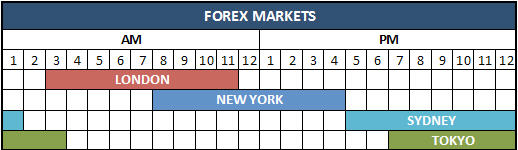
\includegraphics[width=0.8\textwidth]{images/ventana}
        \caption{Ventana de tiempo de los mercados financieros}
        \label{fig:forex_markets_hours}
    \end{center}
\end{figure}

\noindent Además se puede ver en tiempo real el estado de cada centro de forma
online\footnote{\url{http://forex.timezoneconverter.com/?timezone=GMT&refresh=5}}.

\vspace{1cm}
\noindent\textbf{Obteniendo Data}\\

Existen varias plataformas web (software) para para acceder a Forex, y cada uno
están regulados por distintas entidades:
\begin{itemize}
 \item Oanda \footnote{\url{http://www.oanda.com/lang/es/}}: es uno de los
\emph{brokers} estado unidense más antiguos (1996).  Su servicio de Trading
Forex está habilitado el año 2001. Cuentan con un software llamado fxTrade que
posee dos modalidades: dinero virtual y dinero real. Para la cuenta de
demostración se puede solamente probar con dinero virtual. La data tick es
completamente gratis, pero para acceder a ella es necesario tener una cuenta en
Oanda que tenga al menos \$1000 USD.
 \item MB Trading \footnote{\url{http://www.mbtrading.com/}}: otro broker
estadounidense, ofrece data tick desde el año 2011, la cual detalla solamente
el top del order book, es decir, el mínimo ask y máximo bid sin incluir el
volumen. Posee una herramienta online y de escritorio (ctrade en windows) para
acceder a la data histórica. Uno de los contra es que la data está dividida en
días y si uno quiere descargar cierto período de días, hay que concatenar la
data a mano.
 \item Gain Capital: fue fundada en 1999, y fue uno de los primeros
desarrolladores de trading forex online. Posee una cuenta \emph{mini} de \$250
USD con la cual se pueden operar transacciones
\footnote{\url{http://www.forex.com/uk/index.html}}, sin embargo la data histórica
está disponible en directorios online y se puede descargar desde el 2000 por
semanas \footnote{\url{http://ratedata.gaincapital.com/}}. Cabe destacar que los primeros
años esta empresa solamente soportaba trading en los stock más importantes.
 \item Dukascopy \footnote{\url{http://www.dukascopy.com/}}: es uno de los brokers
más reconocidos actualmente. Es una institución financiera constituida en
Suiza, que desde el 2010 se convierte oficialmente en un banco. Para crear una
cuenta de trading, exige mínimo \$1000 USD, posee una plataforma online y una
aplicación de escritorio (JForex), con las cuales se puede interactuar de forma
simple para acceder a la data histórica de forma gratuita.
\end{itemize}

Para esta memoria se usó la plataforma JForex de Dukascopy.

\section{Series de tiempo financiera}

La mayoría de los fenómenos que se estudian en su componente temporal, deben
tomar en cuenta la dinámica de los proceso con la finalidad tener una
comprensión general del mismo. Una herramienta útil en dicho objetivo es el
análisis de series de tiempo. Una serie de tiempo, es una secuencia de datos
indexados por su marca temporal. Se pueden presentar casos de series de tiempo
en una multitud de disciplinas como ingeniería, sociología, economía, finanzas
por solo mencionar algunas de ellas.

El propósito fundamental es mostrar las técnicas que permitan hacer inferencias
del proceso en estudio incluyendo su predicción. Esto se logra estableciendo
modelos probabilísticos hipotéticos que representen a los datos; y en
consecuencia, se lleva a cabo el proceso de ajuste, que incluye desde la
estimación hasta la predicción, una vez que se ha determinado un modelo
satisfactorio para la muestra de datos~\cite{box2011time}
~\cite{vandaele1983applied}. 

En particular, el análisis de una serie de tiempo financiera puede enfocarse en
analizar de forma teórica y práctica la valoración de cierto instrumento en el
tiempo, como también los volúmenes transados, etc. Lo que se intenta es modelar
la incertidumbre generada por las características propias de este fenómeno
~\cite{tsay2005analysis}. 

Las características diferenciadoras han propiciado numerosos trabajos en las
áreas de econometría y economía financiera desde los años 60. Es por ello que,
en el área financiera las evidencias sobre patrones ha conducido a la
formulación de distintos modelos matemáticos.

\subsection{Descripción de serie financiera}

Una tendencia en el análisis de las series financieras, es el seguimiento del
precio de un instrumento en el tiempo.
%Las series de tiempo financieras, se basan en el estudio del precio de un
%instrumento financiero en el tiempo. 
Existen varios tipos de precios que se pueden analizar, por un lado están los
indicadores que se utilizaron en los primeros estudios formales, los cuales
mostraban información al respecto de los precios de: \emph{apertura},
\emph{cierre}, \emph{el más bajo}, \emph{el más alto}, \emph{promedio}. Esos
datos estaban orientados a tomar métricas respecto a valores que resumían los
cambios de precio de un instrumento en un día. Una muestra gráfica de esta
información se puede ver en la figura \ref{fig:microsoft} \footnote{Imagen
tomada de \url{http://www.stockrageous.com/}}
%con estos datos quedaban gráficos como el siguiente:

\begin{figure}[h!t]
    \begin{center}
        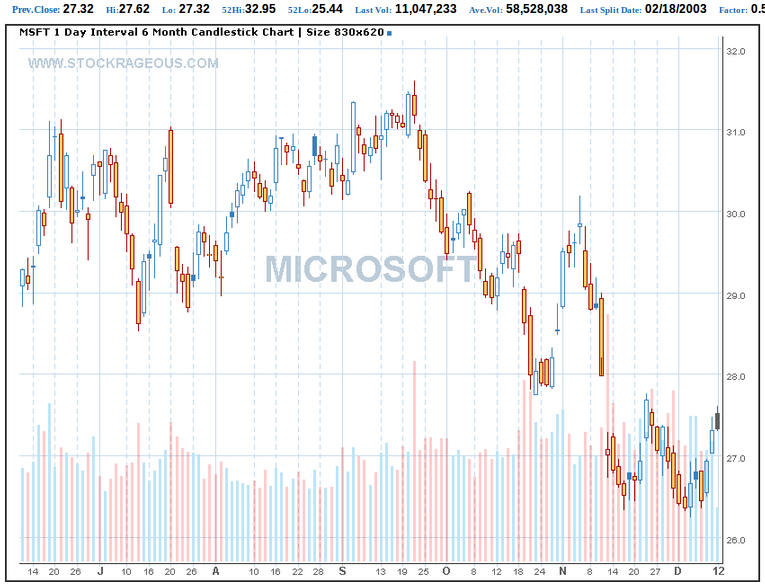
\includegraphics[width=0.7\textwidth]{images/microsoft}
        \caption{Información de los precios de microsoft en la bolsa.}
        \label{fig:microsoft}
    \end{center}
\end{figure}

Con esa información se realizaban \emph{estudios técnicos}
~\cite{taylor1992use}, los cuales proporcionaban pronósticos de tendencias (como
subir o bajar de precio), basándose en la inspección visual y búsqueda de
patrones en los precios anteriores del instrumento. 

Sin embargo la data estudiada actualmente corresponde a data \emph{intra
diaria}, la cual reside en los valores específicos en que se compró o vendió
algún instrumento.  Ese precio se conoce como el \emph{last price}, y
corresponde al valor específico con el cual se realizó la transacción. La forma
de como se efectúa este evento es mediante los \emph{market} o \emph{limit
orders}, donde existe una cola de compras o ventas obtenidas mediante los
\emph{limit orders} y que cuando se cumpla la condición asociada (de vender o
comprar a cierto precio), se realiza la transacción y se registra dicho
\emph{last price}. Recopilando esa información, se puede generar una secuencia
temporal de los \emph{last prices}. 
%Estudios prácticos de estas series \cite{biais2012empirical},
%generalizan su gráfica con forma de \emph{U},

A través de la historia, estas interacciones se realizaban personalmente en las
bolsas de comercio, en los llamados \emph{floor market}
~\cite{jain2005financial}, sin embargo con el avance de las tecnologías, se han
implementado distintas plataformas de \emph{trading electrónico}: un método de
negociación de instrumentos financieros por medios electrónicos
~\cite{weston2002electronic}. Estas tecnologías se utilizan para reunir a
compradores y vendedores a través de plataformas de comercio electrónico, como
por ejemplo: National Association of Securities Dealers Automated Quotation
(NASDAQ), New York Stock Exchange (NYSE), etc. Tomando en cuenta las nuevas
frecuencias de aparición de datos, en el orden de fracción de segundos, se
torna difícil manejar los datos de forma humana, es por esta razón que es
necesario realizar análisis cuantitativos mediante algoritmos computacionales.

%Las series financieras de alta frecuencia tienen características particulares
%en relación a otras series, como son: 
%\begin{itemize}
%	\item Frecuencia: la frecuencia en la observación de los datos es mayor que
%en otro tipo de series de tiempo, en el orden de fracción de segundos.
%	\item Heterocedasticidad: ocurre cuando la varianza de las perturbaciones
%no es constante a lo largo de las observaciones.  Este factor hace inadecuados
%los modelos desarrollados para series estacionarias.
%	\item No estacionalidad: en muchos casos la media y varianza se presentan
%como no estacionarias.
%	\item Información oculta: se pueden encontrar distintos tipos de patrones a
%diferentes niveles de escala.
%\end{itemize}

\subsection{Serie de tiempo Forex}

\section{High Frequency Trading}

Esta sección busca detallar componentes de un sistema de trading electrónico, 
conceptos de funcionamientos, actores, etc.

\subsection{Sistema de trading y componentes}
Un sistema electrónico de trading es una infraestructura que permite el ingreso
de órdenes, generación y envío de datos financieros con precios, y el match de
dichas órdenes en base a un criterio predefinido.

Una de las ventajas de este tipo de sistema por sobre sus antecesores, es su
diseño robusto, ya que permiten automatizar el proceso, entregar confiabilidad,
escalabilidad, seguridad y performance: capacidades que luego de cierto volumen
de son imposibles de realizar de forma manual.

No existe una estructura estándar en los distintos mercados mundiales para
sistemas de trading, generalmente se emplea una arquitectura compuesta por los
siguientes elementos:
\begin{itemize}
 \item Interfaz de ingreso de órdenes del lado del servidor, la cual implementa
un protocolo propietario o estándar.
 \item Terminales de trading, con un \emph{trader} humano operando u otros
sistemas, que se comunican mediante cierto protocolo y se conecta a la
interfaz. Estas son conocidas como frontend si el usuario es una persona, o un
Order Management System (OMS).
 \item Matching Engine, el cual recibe órdenes de compra y venta según un
criterio predefinido las empareja, juntando así compradores y vendedores de un
mismo activo que se ponen de acuerdo en un precio y una cantidad.
 \item Interfaz de Market Data, que presenta los precios disponibles en el
sistema como referencia, e informa de nuevas operaciones realizadas, a la que
se conectan distintos \emph{vendors} de data y las terminales y sistemas antes
mencionados.
 \item Sistema de \emph{backoffice} para hacer seguimiento de las operaciones
concertadas, la realización de \emph{allocations} o \emph{giveups}, si el
mercado y el regulador lo permitieran, y el seguimiento de posiciones, status
de \emph{clearing} y liquidación de transacciones.
\end{itemize}

Generalmente estos elementos se suelen agrupar también en \emph{frontoffice}
(actividades relacionadas al trading) y en \emph{backoffice} (actividades
relacionadas al \emph{clearing} y \emph{settlement} de las transacciones,
mantenimiento de garantías y márgenes, y seguimiento de las operaciones
realizadas).

Otra clasificación usada también es la de \emph{pre-trade}, \emph{trade} y
\emph{post-trade}, para separar las actividades en función de su ubicación
relativa a la concreción de la transacción.


\subsection{Órdenes, Order books y lógica de matching}

En \emph{HFT}, según el mercado y la autorización del regulador, existen
distintos tipos de órdenes, siendo las más comunes detalladas a continuación:
\begin{itemize}
 \item \emph{Market order}: orden para comprar o vender cierta cantidad de un
 activo al precio disponible de Mercado, recorriendo el \emph{order book} hasta
 completar la cantidad total. De esta operación surge un precio promedio
 ponderado compuesto por las cantidades parciales multiplicadas por el precio
 de cada una de ellas, para determinar el precio de ejecución.
 \item \emph{Limit order}: orden ingresada con precio y cantidad, si hubiera
 disponible contra-parte se ejecuta la porción de la cantidad disponible y el
 resto queda guardado en el libro a ese precio. 
 \item Orden tipo Market to limit: orden para comprar o vender a cierta
 cantidad de un activo al precio de mercado, si la cantidad total no se
 ejecuta, el restante queda en el libro como orden tipo \emph{limit} al precio
 ejecutado.
 \item \emph{Stop limit order}: orden que se ingresa con 2 precios, precio de
 stop y precio de limit, cuando se alcanza el precio de stop (otro participante
 opera a ese precio en el mercado), se ejecuta una orden de compra o venta por
 el precio \emph{limit}.
 \item Orden Iceberg: orden para comprar o vender cierta cantidad de un activo
 a un precio específico. Este tipo de orden es generalmente utilizado por
 inversores institucionales u operadores que desean hacer una operación por una
 cantidad importante y que no quieren que esta provoque un movimiento de precio
 desfavorable.
\end{itemize}

A su vez es posible combinar los tipos de órdenes disponibles con un parámetro
de duración:
\begin{itemize}
 \item \emph{Fill or Kill}: la orden se ingresa en el Mercado y si no puede llenarse
 automáticamente se cancela, no quedando en el libro.
 \item \emph{Day}: la orden queda en el mercado por el día, pero al cerrar la rueda,
 según el horario definido esta expira.
 \item \emph{Good till canceled}: con o sin fecha definida: ciertos mercados permiten
 el modificador \emph{DATE} que da la posibilidad de indicar hasta qué fecha la orden
 podrá estar en el libro hasta ser ejecutada hasta la fecha especificada o
 indefinidamente. 
\end{itemize}

Todos los mercados cuentan con un \emph{order book} o libro de órdenes, que ha
evolucionado desde una pizarra donde se escribían con tiza los precios y
cantidades ofertadas por los agentes a sistemas electrónicos de bases de datos
que almacenan las ofertas de los clientes.


\subsection{Tipo de mercados: brokers/dealers y acceso directo}

Actualmente la operación en mercados puede simplificarse en dos modalidades:
que la orden de un cliente ingresada a través de un \emph{broker} se ejecute
contra inventario del \emph{broker/dealer}, o que esta sea enviada a un libro
central, donde las órdenes son \emph{matcheadas} entre sí según los criterios y
tipos.

Esta modalidad es conocida como acceso directo al mercado y en principio es más 
transparente para los inversores finales ya que siempre se está operando contra 
el precio de mercado.


\subsection{Interfaces únicas y protocolos}
A medida que los nuevos sistemas electrónicos fueron naciendo en la década de
los 80, primero como una herramienta para diseminar precios, mientras las
operaciones todavía seguían concretándose por teléfono, y luego a fines de los
90 cuando se avanzó hacia una migración completa a lo electrónico, mediante la
desaparición del piso, el lenguaje de comunicación o protocolo utilizado por
estos sistemas era específico y distinto para cada uno de ellos.

Los sistemas informáticos que realizan la labor de facilitar el comercio de
instrumentos financieros, son los llamados \emph{Electronic communication
networks} (ECN).  Se crearon en 1998, año que fueron autorizados por la
\emph{Securities and Exchange Commission} y se basaron en los protocolos
definidos en la Financial Information Exchange~\cite{mcandrews2000emergence}.
La SEC~\cite{hasbrouck2004economic} es una organización estadounidense creada
en 1933, y tiene la responsabilidad de velar por el cumplimiento de las leyes
federales las bolsas de valores. Un caso emblemático, fue el 6 de mayo del
2010, fecha en la cual ocurrió el \emph{Flash-Crash}~\cite{arndt2011high}, dio
a lugar a una quiebra financiera estadounidense en el que el índice \emph{Dow
Jones Industrial Average} se desplomó un 9\%. 

\subsection{Protocolo Financial Information eXchange}
Financial Information eXchange (FIX) es un protocolo de mensajes para el
comercio de instrumentos financieros. FIX se utiliza ampliamente para la
comunicación automática entre los participantes del intercambio de
instrumentos, y especifica como son los mensajes para crear órdenes de compra y
venta y consultar cotizaciones de instrumentos, entre otros. Este protocolo es
el que hay que utilizar para comunicarse con prácticamente todos los mercados
financieros de manera electrónica.

FIX fue creado en 1992, y durante esa fecha ha ido evolucionando, lo que ha
generado distintas versiones, agregando diferentes mensajes y campos para
acomodar las funciones requeridas por los participantes de todo el mundo. La
versión del protocolo se divide en dos: mensaje (por ejemplo FIX 5.0) y el
protocolo de transporte (FIXT 1.1).
El formato FIX es un formato textual, donde cada mensaje es una linea de la
forma:
\vspace{0.5cm}
\begin{verbatim}
        8=FIX.5.0|9=65|35=A|49=SERVER|56=CLIENT|34=177|
        52=20090107-18:15:16|98=0|108=30|10=062|
\end{verbatim}
\vspace{0.5cm}

\noindent Donde se menciona el tipo de mensaje (campo 35), checksum (10), versión de
FIX(8), etc. FIX es un protocolo abierto y gratuito, ya que es solo la
especificación de los mensajes y de los campos mínimos. Existen distintas
implementaciones del protocolo como QuickFIX/C++, QuickFIX/Python, etc.

\subsection{Eficiencia: descubrimiento de precios, liquidez y volatilidad}

\emph{Price discovery}: proceso por el cual las voluntades de compra y venta de
activos por distintos actores, ofreciendo un precio que - en teoría - lleva
descontada toda la información disponible sobre el activo, permite establecer
el valor en este momento.

\emph{Liquidez}: es la propiedad por la cual es posible adquirir o desprenderse
de un activo con relativa sencillez, sin altos costos y sin que la operación
modifique el precio de manera significativa.

\emph{Volatilidad}: medida de variación de los precios en ambas direcciones de
un activo en un intervalo dado. Puede estar medida en precio exacto o en
porcentaje.


\subsection{Definición de High Frequency Trading}

Se puede definir un mercado de alta frecuencia en base al estudio hecho por el
Boston Consulting Group para la SEC como: \emph{una estrategia que se apoya
en la rotación de pequeñas posiciones muy rápidamente mediante el ingreso de
órdenes de compra o venta de activos, basadas en la detección de ineficiencias
o patrones de mercado}~\cite{genccay2001introduction}.

Como indica el estudio, la tecnología y la velocidad son características claves
que requiere de sistemas automatizados capaces de identificar oportunidades
e ingresar grandes cantidad de órdenes y operarlas a velocidades medidas en
milisegundos.

Con el paso del tiempo y la implementación de distintos sistemas de trading
electrónico, la frecuencia de la data aumentó, pasando de minutos a fracciones
de segundos.  En estos sistemas se define como unidad atómica de información un
\emph{Tick}. Un \emph{Tick} especifica una gran cantidad de parámetros como la
marca temporal, precio, cantidad transada, etc. Los datos de alta frecuencia
son un conjunto de datos de reportes detallados sobre la actividad y movimiento
efectuados sobre un instrumento. Se reúne la información de los ticks con
cierto intervalo de tiempo, el cual para este tipo de series es variable. En la
literatura se puede encontrar más de un término para definir este fenómeno
~\cite{ei2007quantitative}, como (ultra-)high-frequency data, microstructure
data, entre otros. 

%Dada la sofisticación de esta actividad, los principales actores de estos
%sistemas son \emph{brokers/deales} con un avanzado desarrollo de su tecnología
%interna. Este tipo de actores suelen ser al mismo tiempo \emph{market makers}
%de los mercados donde ejecutan este tipo de estrategias, por lo que el
%beneficio obtenido es apalancado por los rebates o concesiones económicas que
%el mercado les hace.

El objetivo de este ingreso tan rápido de órdenes es capturar el \emph{spread}
de compra venta antes que otros actores, \emph{spreads} que en muchos casos son
décimas de centavos, pero que la alta velocidad y cantidad de operaciones hacen
rentable el negocio.

Generalmente este tipo de actividad hace que las posiciones solo sean
mantenidas durante el mismo día en que son abiertas, por lo que implica la
necesidad de un capital importante o una gestión de riesgo más profunda que si
se tomaran posiciones con un horizonte de tiempo más amplio.

Se puede decir que dos factores claves han dado pie al surgimiento y
crecimiento de esta tendencia: la modernización de la estructura de los
mercados de capitales y el desarrollo de la tecnología informática. Desde el
punto de vista de mercados los factores puntuales han sido:
\begin{itemize}
 \item La \emph{electronización} de los mercados: el hecho que los mercados
 sean electrónicos y el \emph{matching} automático, permiten ganar en
 velocidad, eficiencia y escala. Esto permite procesamiento de \emph{Market
 Data} y el ingreso de órdenes en base a patrones o algoritmos. 
 \item La decimalización: en un principio los precios de las equities se
 expresaban con fracciones, esto es, una acción de USD podía valer 3 y 4/7. La
 decimalización hizo posible pasar el formato de los precios a decimales, lo
 que los hizo más fácilmente operables por programas automatizados. Esta
 iniciativa permitió abrir los precios y generar spreads más finos.
 \item La competencia entre los distintos tipos de mercados permitió que
 estrategias más sofisticadas pudieran ser implementadas, y que los
 participantes pudieran hacer que los mercados permitieran el uso de tecnología
 de automatización de forma cada vez más avanzada.
 \item El acceso directo al mercado y el uso del \emph{order book} central
 permite que una orden ingresada pegue directamente sobre el conjunto de todas
 las órdenes disponibles, permitiendo impactar sobre todo el conjunto del
 mercado para ese activo y no de forma fragmentada como podría ser contra el
 inventario de un dealer.
\end{itemize}

Y los avances en tecnología como:
\begin{itemize}
 \item Aumento en la velocidad de transferencia en redes de datos, en varios
órdenes de magnitud: de 100 Mbit/seg, a 1Gb/seg, luego 10 Gb/Seg y finalmente
Infiniband internamente.
 \item Aumento de capacidad de procesamiento sujetos a la ley de moore.
\end{itemize}

Estos cambios tecnológicos permitieron que fuera más fácil que algoritmos
avanzados pudieran procesar gran cantidad de datos, por ejemplo: cálculo de
escenarios, correlaciones entre miles de activos en tiempo real y gestión del
riesgo lo suficientemente rápido como para que el tiempo entre esta actividad y
el envió de una orden al mercado no significara un riesgo de quedar desfasado
del cambio que se acababa de producir en el precio o cantidad.

%La velocidad es un factor tan importante que los actores de este segmento
%llegan incluso a arrendar espacio de rack en los datacenters de los mercados
%para estar más cerca del sistema central de procesamiento, ganando así unos
%microsegundos en el tiempo de latencia hasta llegar al Matching Engine. 

En esto la velocidad es clave, ya que poder procesar el \emph{book} e ingresar
miles de órdenes antes que un competidor, es lo que da la ventaja competitiva.
La combinación de tecnología con algoritmos de procesamiento del \emph{book} e
ingreso de ordenes permite adelantarse a los cambios y poder posicionarse al
resto de los participantes. 
 
Existen una serie de análisis del punto de vista económico y financiero que
concluyen que los HFT son beneficiosos o nocivos para los mercados, sin embargo
este tipo de análisis no es de interés para esta memoria ya que lo relevante de
este tipo de mercado es la cantidad de datos que generan y su naturaleza
temporal.


        \chapter{Antecedentes}
        \label{ch:backgound}
        En esta sección se presentarán los fundamentos matemáticos de dos modelos
usados en el estudio de series de tiempo, las condiciones que deben cumplirse y 
cómo serán aplicados a la predicción en el mercado FOREX. 

\section{Series de tiempo estacionarias}
Una serie de tiempo $\{y_{t_n}\}, n \in \mathbf{Z}$ se dice estrictamente
estacionaria cuando el comportamiento probabilístico de cada colección
correlativa de valores $\{y_{t_1},y_{t_2},\dots,y_{t_L}\}$ es idéntico a otro
set correlativo desplazado en el tiempo, más preciso: 
\[ P\{y_{t_1} \leq
c_1,\dots,y_{t_L} \leq c_L\} = P\{y_{t_1+h} \leq c_1,\dots,y_{t_L+h}
\leq c_L\}
\quad \forall L \in \mathbb{N}, \forall h \in \mathbb{Z}\] \noindent donde
$c_1,\dots,c_L$ son constantes.

Esta definición es muy fuerte y difícil de evaluar desde un set de datos único
\cite{shumway2010time}.

La versión débil de esta definición impone condiciones solo en los dos primeros
momentos.

Una serie de tiempo débilmente estacionaria es un proceso que su media,
varianza y autocovarianza no cambian en el tiempo:

\begin{eqnarray*}
E(Y_t) &=& \mu  \quad \forall t \in \mathbb{N} \\ E(Y^2_t) &=&
\sigma^2  \quad \forall t \in \mathbb{N} \\
\lambda(s,t)&=&\lambda(s+h,t+h) \quad \forall s,t \in \mathbb{N},
\forall h \in \mathbb{Z}
\end{eqnarray*}

\noindent con $\lambda(s,t) = E[(y_s-\mu)(y_t - \mu)]$.

\section{Vector AutoRegressive (VAR)}

VAR es un marco general que describe el comportamiento de un set $l$ de
variables endógenas como una combinación lineal de sus últimos $p$ valores. En
la literatura se nombra como variable endógena $y_t$, y como exógenas las
variables explicativas de regresión $y_{t-1}, \dots, y_{t-p}$.  Esas $l$
variables en el tiempo $t$ son representadas por el vector $y_t$ como:

\begin{equation}
\label{eq:variables}
\mathbf{y}_t = 
\begin{bmatrix} y_{1,t} \\
y_{2,t} \\
\vdots \\
y_{l,t}
\end{bmatrix}
\end{equation}
\noindent Donde $y_{j,t}$ corresponde a la serie de tiempo $j$ evaluada en el
tiempo $t$.

El modelo VAR(p) describe el comportamiento de una variable dependiente en
términos de sus propios valores rezagados y el de otras variables en el
sistema. El modelo con $p$ rezagos se formula como el siguiente:

\begin{equation}
\label{eq:var}
 \mathbf{y}_t = \phi_1 \mathbf{y}_{t-1}  + \dots +   \phi_p\mathbf{y}_{t-p}
 + \mathbf{c} + \mathbf{\epsilon}_t, \qquad t=p+1, \dots, N
 \end{equation}

\noindent donde ${\phi_1,\dots,\phi_p}$ son $l \times l$ matrices de
coeficientes reales, $\mathbf{\epsilon}_{p+1},\dots,\mathbf{\epsilon}_N$ son
términos relacionados al error, $\mathbf{c}$ es un vector constante y $N$ es el
número total de muestras.

La matriz VAR tiene la siguiente forma:

\begin{equation}
 \label{eq:varmatrix}
 \resizebox{0.9\hsize}{!}{$%
               \underbrace{ \begin{bmatrix}
               \quad \\
               \mathbf{y}_{p+1} &
               \mathbf{y}_{p+2} &
               \dots & 
               \mathbf{y}_N \\
               \quad
               \end{bmatrix}}_{\substack{ \mathbf{B}\\l \times (N-p)}}   
= 
                \underbrace{\left[ 
                \begin{array}{ccccc}
                \quad & \quad & \quad & \quad & \quad \\
                \phi_1  & \phi_2 & \cdots & \phi_p & \mathbf{c} \\  
                \quad &\quad & \quad & \quad & \quad
               \end{array} 
               \right]}_{\substack{ \mathbf{X}\\ l \times (l \times p + 1 )}}
\underbrace{\begin{bmatrix}
   \mathbf{y}_{p}  & \mathbf{y}_{p+1} & \dots    & \mathbf{y}_{N-1}\\
   \mathbf{y}_{p-1}  & \mathbf{y}_{p} & \dots    & \mathbf{y}_{N-2}\\
   \vdots        & \vdots   & \ddots   & \vdots\\
   \mathbf{y}_{1} & \mathbf{y}_{2}   & \dots    & \mathbf{y}_{N-p}\\
   1 & 1   & \dots    & 1 
   \end{bmatrix}}_{\substack{ \mathbf{A}\\ (l\times p +1 )(N-p)}}
+
\underbrace{\begin{bmatrix}
                \quad \\
              \mathbf{\epsilon}_{p+1}  & 
              \mathbf{\epsilon}_{p+2}  & 
              \dots                & 
              \mathbf{\epsilon}_N \\
              \quad
             \end{bmatrix}}_{\substack{\mathbf{E}\\l \times (N-p) }} 
$}
\end{equation}
%$
\section{Integración y Cointegración}
Un proceso estocástico $\mathbf{Y}$ es llamado integrado de orden $d$, si
después de diferenciar $d$ veces, se obtiene una variable I(0) (proceso
estacionario):

\[
(1-L)^d \mathbf{Y} \sim \text{I(0)}
\]
\noindent donde I(0) es una serie de tiempo estacionaria y $L$ es el operador de rezago, i.e,
\[
(1-L)\mathbf{Y} = \Delta \mathbf{Y}
\]
\noindent donde $\Delta \mathbf{Y}(t) = \mathbf{Y}(t)  -\mathbf{Y}(t-1) \quad \forall t $.

Definamos $\mathbf{Y}_t = \{\mathbf{y}^1, \dots, \mathbf{y}^l\}$ como un set de $l$ series de tiempo estacionarias 
I(1) que se dice que es cointegrada si un vector,
$\beta=[\beta(1),\dots,\beta(l)]^\intercal \in \mathbb{R}^l$  existe tal que la serie de tiempo, 

\begin{equation}
 \mathbf{Z}_t:= \beta^\intercal \mathbf{Y}_t = \beta(1) \mathbf{y}^1 + \dots + \beta(l) \mathbf{y}^l \sim
  \text{I(0)}
  \end{equation}

En otras palabras, un set de variables I(1) se dice que son cointegradas si
existe una combinación lineal de ellas que es I(0).

El siguiente ejemplo~\cite{johansen1995} ayuda a ilustrar el significado de
$\beta$:

\textbf{Ejemplo:}

Si tenemos un proceso 2-dimensional $\mathbf{X}_t$, $t=1,\dots,T$ por:

\begin{eqnarray*}
\mathbf{X}_{1t} &=& \sum_{i=1}^t \epsilon_{1i} + \epsilon_{2t} \\
\mathbf{X}_{2t} &=& a \sum_{i=1}^t \epsilon_{1i} + \epsilon_{3t} 
\end{eqnarray*}

Como $\mathbf{X}_{1t}$ y $\mathbf{X}_{2t}$ son procesos I(1) y existe un vector
$\beta = [a -1]$ tal que:

\[
\beta^\intercal \mathbf{X}_t = a \mathbf{X}_{1t} -\mathbf{X}_{2t} = 
a\epsilon_{2t} - \epsilon_{3t} \sim \text{I(0)}
\]

entonces, ambos procesos se dicen que están cointegrados. Si agregamos un proceso I(0)
$\mathbf{X}_{3t} = \epsilon_{4t}$ encontramos que existen dos vectores de cointegración: 
$\begin{bmatrix}a &-1& 0\end{bmatrix}$ y $\begin{bmatrix}0
&0&1\end{bmatrix}$ como:

\[
\beta^\intercal \mathbf{X}_t = 
\begin{bmatrix}
a & -1 & 0 \\
0 & 0 & 1
\end{bmatrix} 
\begin{bmatrix} 
\mathbf{X}_{1t} \\
\mathbf{X}_{2t} \\
\mathbf{X}_{3t}
\end{bmatrix} = 
\begin{bmatrix}
a\epsilon_{2t} - \epsilon_{3t} \\
\epsilon_{4t}
\end{bmatrix}
\]

Este ejemplo muestra como los vectores de cointegración describe la relación
estable entre los procesos a través de relaciones lineales que son más
estacionarias que el proceso original.

Un ejemplo clásico de cointegración, en términos no matemáticos, es el de los
borrachos cuando se amarran con una cuerda (dos pares de divisas), no se sabe
qué  dirección tomarán (alza o baja), lo único que se sabe es que se mueven
juntos con una desviación máxima del tamaño de la cuerda (cointegración).  Por
tanto no podemos apostar a que vayan en una dirección o en otra como se basa el
trading direccional, solo se puede apostar que una vez que se separen (lo
máximo que de la cuerda) acabarán otra vez juntos en algún momento.

Es importante entender que cointegración no es correlación. Correlación es una
relación a corto plazo de movimiento de los precios. Mientras que la
cointegración significa que los precios mueven juntos. La cointegración se
refiere a la relación equilibrada entre varias series de tiempo, por ejemplo,
considerando los precios de divisas, aunque los precios de cada una cambie de
forma aleatoria en ciertos periodos de tiempo, finalmente retornan al
equilibrio, y su desviación será estacionaria.

\section{Vector Error Correction (VEC)}

El modelo VEC es una forma especial de un modelo VAR para variables I(1) que
están también cointegradas. El modelo VEC es obtenido reemplazando
$\Delta \mathbf{y}_t = \mathbf{y}_t - \mathbf{y}_{t-1}$ en ecuación
(\ref{eq:var}). El modelo VEC es expresado en términos de diferencias,
tiene un término de corrección de error y tiene la siguiente forma:

\begin{equation}
 \label{eq:vec}
  \Delta \mathbf{y}_t = 
   \underbrace{ \Omega\mathbf{y}_{t-1}}_\text{Término de corrección de error} + 
    \sum_{i=1}^{p-1}
    \phi_i^* \Delta \mathbf{y}_{t-i}  + \mathbf{c} + \mathbf{\epsilon}_t \quad ,
    \end{equation}

    \noindent donde las matrices de coeficientes $\Omega$ y $\phi_i^*$ son
    funciones de matrices $\phi_i$ (mostradas en la ecuación (\ref{eq:var})) de
    la siguiente forma:

    \begin{eqnarray*}
    \phi_i^* &: =& -\sum_{j=i+1}^{p} \phi_j \\
    \Omega &: =& -(\mathbb{I}-\phi_1-\dots-\phi_p) 
    \end{eqnarray*}

    La matriz $\Omega$ tiene las siguientes propiedades:
    \begin{itemize}
    \item Si $\Omega = 0$ no hay cointegración 
    \item Si $rank(\Omega)=l$ i.e full rank, entonces la serie de tiempo no es I(1) pero es estacionaria
    \item Si $rank(\Omega)=r,\quad 0 < r < l$ entonces, hay cointegración 
    y la matriz $\Omega$ se puede expresar como $\Omega =
    \alpha \beta^\intercal$, donde $\alpha$ y $\beta$ son $(l \times r)$
    matrices y $rank(\alpha)=rank(\beta)=r$.

    La columna de $\beta$ contiene los vectores de cointegración y la fila de
    $\alpha$ corresponde a los vectores de ajuste. $\beta$ se obtiene a través
    el procedimiento de Johansen~\cite{johansen1988} mientras que $\alpha$ debe
    ser determinado como variable en el modelo VEC.

    Cabe observar que la factorización de la matriz $\Omega$ no es única ya que por cada
    $r \times r$ matriz no singular $H$ tenemos:

\begin{eqnarray*}
\alpha \beta^\intercal &=& \alpha \mathbf{HH^{-1}} \beta^\intercal\\
&=&(\alpha\mathbf{H})(\beta(\mathbf{H}^{-1})^\intercal)^\intercal \\
&=& \alpha^*(\beta^*)^\intercal
\end{eqnarray*}

\noindent con $\alpha^* = \alpha\mathbf{H}$ y $\beta^* =
\beta(\mathbf{H}^{-1})^\intercal$.

Por lo tanto, para obtener valores únicos, son requeridas más restricciones
para el modelo.

\end{itemize}

Si existe cointegración, entonces la ecuación (\ref{eq:vec}) puede ser escrita:
\begin{equation}
 \label{eq:vecfull}
  \Delta \mathbf{y}_t = \alpha \beta^\intercal\mathbf{y}_{t-1} 
   + \sum_{i=1}^{p-1} \phi_i^*\Delta
   \mathbf{y}_{t-i}  + \mathbf{c} + \mathbf{\epsilon}_t \quad ,
   \end{equation}

   \noindent que es un modelo VAR pero para series de tiempo diferenciadas.

La forma matricial del modelo VEC es:
\begin{equation} \label{eq:vecmatrix}
\resizebox{0.9\hsize}{!}{$%
\underbrace{
                \left[ \begin{array}{ccc}
               \quad & \mathbf{\Delta y}_{p+1} & \quad \\ 
               \quad & \mathbf{\Delta y}_{p+2} & \quad \\
               \quad & \vdots & \quad \\ 
               \quad & \vdots & \quad \\  
               \quad & \mathbf{\Delta y}_N & \quad 
               \end{array} \right]}_{\substack{\mathbf{B}\\ (N-p) \times l }} =
   \underbrace{\left[ 
    \begin{array}{cccccc}
     \quad & \quad & \quad & \quad & \quad & \quad \\
     \alpha & \phi_1^*  & \phi_2^* & \cdots & \phi_{p-1}^* & \mathbf{c} \\  
     \quad &\quad &\quad & \quad & \quad & \quad
     \end{array} 
      \right]}_{\substack{ \mathbf{X}\\ (l(p-1)+r+1) \times l}}
\underbrace{\begin{bmatrix} 
   \beta^\intercal \mathbf{y}_{p} & 
   \beta^\intercal \mathbf{y}_{p+1}&
   \cdots & \beta^\intercal \mathbf{y}_{N-1} \\
   \mathbf{\Delta y}_p & \mathbf{\Delta y}_{p+1} & \cdots 
   & \mathbf{\Delta y}_{N-1} \\ 
   \vdots & \vdots & \ddots & \vdots \\
   \mathbf{\Delta y}_2 & \mathbf{\Delta y}_{3} & \cdots 
   & \mathbf{\Delta y}_{N-p+1} \\ 
   \end{bmatrix}}_{\substack{\mathbf{A} \\ (N-p) \times (l \times (p-1)+r+1) }}
+
\underbrace{\begin{bmatrix}
              \quad &\mathbf{\epsilon}_{p+1} & \quad \\ 
              \quad &\vdots & \quad\\ 
              \quad & \vdots & \quad\\
              \quad & \vdots & \quad\\
              \quad &\mathbf{\epsilon}_N & \quad
             \end{bmatrix}}_{\substack{\mathbf{E}\\ (N-p) \times l }} 
$}
\end{equation}
%$
Los parámetros de los modelos VAR y VEC mostrados en la ecuación
(\ref{eq:varmatrix}) y (\ref{eq:vecmatrix}) pueden ser resueltos usando
técnicas de regresión estándar, como mínimos cuadrados ordinaria (OLS por si
sigla en inglés). Sin embargo, la matriz $\mathbf{A}$ es usualmente deficientes
de rank y la solución de OLS no puede ser encontrada.  El método de Ridge
regression (RR) es comúnmente usado en vez de OLS cuando las matrices son mal
condicionadas o deficientes de rango, ya que tiene mejoras en la generalización
en la solución del problema.

\section{Método de Mínimos Cuadrados}
Mínimos Cuadrados, conocido en la literatura en inglés como Ordinary Least Squares (OLS), 
es un método aplicable a la solución de sistemas de ecuaciones lineales. OLS consiste en minimizar
la suma de los errores cuadrados que equivale a minimizar la siguiente expresión:

\begin{equation}
\label{eq:regressionproblem}
\underset{\mathbf{X}}{\text{min}} \quad \| \mathbf{A}\mathbf{\mathbf{X}} - \mathbf{B} \|_2^2
\end{equation}

\noindent para la cual la solución conocida es $\hat{\mathbf{X}}$:

\begin{equation}
\label{eq:MP}
\hat{\mathbf{X}}=\mathbf{A}^{\!\!+}\,\mathbf{B}
\end{equation}

\noindent donde $\mathbf{A}^{\!\!+}$ es la pseudo-inversa de Moore-Penrose que se puede escribir como:

\begin{equation}
\label{eq:pseudoinverse}
\mathbf{A}^{\!\!+}= (\mathbf{A}^{\!\!\top} \mathbf{A})^{-1}\mathbf{A}^{\!\!\top} \, .
\end{equation}

Sin embargo, cuando $\mathbf{A}$ no es full rank, i.e 
$rank(\mathbf{A})=k <  n \leq m$, $\mathbf{A}^\top \mathbf{A}$ es siempre singular
y la ecuación~(\ref{eq:pseudoinverse}) no puede ser usada. Más generalmente,
la pseudo-inversa es mejor calculada usando la descomposición de valor singular compacta (SVD)
de $\mathbf{A}$:

\begin{equation}
    \label{eq:compactsvd}
    \underset{m \times n}{\mathbf{A}}=
    \underset{m \times k}{\mathbf{U_1}} \enskip
    \underset{k \times k}{\Sigma_1} \enskip
    \underset{k \times n}{\mathbf{V}_1^{\top}} \, ,
\end{equation}

\noindent por consiguiente

\begin{equation}
\label{eq:pseudoinversesvd}
\mathbf{A}^{\!\!+} = \mathbf{V}_1 \Sigma_1^{-1} \mathbf{U}_1^\top \, .
\end{equation}


\textbf{Demostración}\quad

Dado que $\mathbf{A}$ es singular el problema mostrado en la ecuación~(\ref{eq:regressionproblem}) 
no tiene solución, la norma mínima dada por la ecuación ~(\ref{eq:MP}) se obtiene resolviendo
el problema equivalente:

\begin{equation*}
\label{eq:proyectorsol}
\mathbf{A \hat{X} = PB} 
\end{equation*}

\noindent donde $\mathbf{P=U_1 U_1^\top}$ es la proyección en Col($\mathbf{A}$).

Dado que $\mathbf{V} = [\underset{(n \times k)}{\mathbf{V_1}} |
\underset{(n \times k)}{\mathbf{V_2}}]$ y $\mathbf{V_1^\top V_2 =
0}$ podemos expresar $\mathbf{\hat{X}} = \mathbf{V_1 x_1 + V_2 x_2}$
con $\mathbf{x_2=0}$ porque $\mathbf{\hat{X}}$ vive en el
$\text{Row}(\mathbf{A})$ dado por $\mathbf{V_1}$, entonces tenemos:

\begin{eqnarray*}
\mathbf{A \hat{X}} &=& \mathbf{PB} \\
\mathbf{U_1 \Sigma_1 V_1^\top \hat{X}} &=& \mathbf{U_1 U_1^\top B} \\
\mathbf{ V_1^\top \hat{X}} &=&  \mathbf{\Sigma_1^{-1} U_1^\top B} \\ 
\mathbf{ V_1^\top V_1 x_1} &=& \mathbf{\Sigma_1^{-1}
U_1^\top B} \\
\mathbf{x_1}&=& \mathbf{\Sigma_1^{-1} U_1^\top B}
\end{eqnarray*}

\noindent desde este resultados podemos obtener $\mathbf{\hat{X}}$ y
por lo tanto la expresión de la pseudo-inversa:

\begin{eqnarray*}
\mathbf{\hat{X}} &=& \mathbf{V_1 x_1} \\
                &=& \mathbf{V_1 \Sigma_1^{-1} U_1^\top B} \\
\mathbf{A^+} &=& \mathbf{V_1 \Sigma_1^{-1} U_1^\top} \, .
\end{eqnarray*}




        \chapter{Graphics Processing Unit}
        \label{ch:gpu}
        \frame{
	%\frametitle{Graphics processing unit}
	\centerline{Graphics processing unit}
}

     
        \chapter{Metodología}
        \label{ch:implementacion}
        %Efficient computation
Dado que los problemas financieros son de corriente de datos, es decir, a
medida que avanza el tiempo aparecen nuevos ticks con información para el
modelo, no es posible incluir todos estos en un solo modelo.  Por lo tanto se
propone una versión online del VECM con la posibilidad de actualizar el modelo
con la nueva data y entregar respuestas en un corto perdiodo de tiempo (mínimo
menor a la frecuencia).

Obtener los vectores de cointegración usando el método de Johansen es también
un procedimiento costoso en cuanto a tiempo computacional. Sin embargo, como
los vectores de cointegración representan la relación a largo plazo entre
series de tiempo, no varian mucho en el tiempo. El algoritmo propuesto obtiene
nuevos vectores de cointegración solamente cuando la relación a largo plazo
cambia. Este cambio se detecta siguiendo en cada paso el cambio del \emph{Mean
Absolute Percentage Error} (MAPE) de los últimos n-ajustes del modelo.

Dado que VECM es un modelo basado en las series tiempo diferenciadas, el MAPE
es obtenido de $\Delta \mathbf{y}$ de la siguiente forma:

\begin{equation}\label{eq:MAPE}
\text{MAPE}[t] = \frac{1}{n} \sum_{i=1}^{n} \left| 
\frac{\Delta \mathbf{y}_{\text{true}}[t-i]-\Delta
\mathbf{y}_{\text{pred}}[t-i]}{\Delta \mathbf{y}_{\text{true}[t-i]}}
\right| \, , 
\end{equation}

\noindent donde $\Delta \mathbf{y}_{\text{true}}$ es el valor actual de la
serie de tiempo diferenciada $\mathbf{y}$ y $\Delta \mathbf{y}_{\text{pred}}$
es su predicción actual.

Cómo este número presenta un promedio el cual puede ser poco representativa de
la muestra se realiza además un estudio de las propiedades estadísticas
clásicas.

\section{Algoritmo Propuesto}

Se propone un algoritmo online con ventanas deslizantes para la predicción del
valor futuro de la cartera de stock FOREX usando el modelo VECM~\ref{alg:proposal}. 

\begin{algorithm}[h!]
\begin{algorithmic}[1]
\REQUIRE $\,$ \\
$\mathbf{y}$: Matriz con $N$ vectores de entrada y $l$ series de tiempo\\
$p$: número de valores anteriores \\
$L$: tamaño de la ventana deslizante ($L<N$) \\
$\text{mean\_error}$: MAPE umbral \\
$n$: puntos de interpolación para calcular el MAPE\\
\ENSURE  $\,$ \\
$\{\Delta \mathbf{y}_{\text{pred}}[L+1],\dots,\Delta \mathbf{y}_{\text{pred}}[N]\}$: predicciones del modelo
\FOR { $i =0$ to $N-L$ }
    \STATE $\mathbf{y}_i \gets \mathbf{y}[i:i+L]$
    \IF {i = 0 }
        \STATE{$v \gets \texttt{getJohansen}(\mathbf{y}_i,p)$}
        \STATE{$[\mathbf{A} \quad \mathbf{B}] \gets
        \texttt{vecMatrix}(\mathbf{y}_i,p,v)$}
    \ELSE
        \STATE{$[\mathbf{A} \quad \mathbf{B}] \gets
        \texttt{vecMatrixOnline}(\mathbf{y}_i,p,v,\mathbf{A},\mathbf{B})$}
        \STATE $\Delta \mathbf{Y}_{\text{true}}[i] \gets \mathbf{B}[-1,:]$
        \STATE $\Delta \mathbf{Y}_{\text{pred}}[i] \gets \mathbf{A}[-1,:] \times \mathbf{X}$
    \ENDIF
    \STATE $\mathbf{X} \gets \text{OLS} (\mathbf{A},\mathbf{B})$
    \STATE $\Delta \mathbf{y}_{\text{true}}[i] \gets \mathbf{B}[-n,:]$
    \STATE $\Delta \mathbf{y}_{\text{pred}}[i] \gets \mathbf{A}[-n,:] \times \mathbf{X}$
    \STATE $e \gets \texttt{mape}(\Delta \mathbf{y}_{\text{true}}, \Delta
    \mathbf{y}_{\text{pred}})$
    \IF {$\texttt{mean}(e) > \text{mean\_error}$}
        \STATE{$v \gets \texttt{getJohansen}(\mathbf{y}_i,p)$}
        \STATE{$\mathbf{A} \gets
        \texttt{vecMatrixUpdate}(\mathbf{y}_i,p,v,\mathbf{A})$}
        \STATE $\mathbf{X} \gets \texttt{OLS} (\mathbf{A},\mathbf{B})$
    \ENDIF
\ENDFOR
\STATE $\text{MAPE} \gets \texttt{mape}(\Delta \mathbf{Y}_{\text{true}}, \Delta
\mathbf{Y}_{\text{pred}})$
\end{algorithmic}
\caption{OVECM: Online VECM}
\label{alg:proposal}
\end{algorithm}

\noindent donde:

\begin{eqnarray}\label{eq:vecmatrix}
 \mathbf{A}&=&
   \begin{bmatrix} 
   \beta^\top \mathbf{y}_{p} & 
   \cdots & \beta^\top \mathbf{y}_{N-1} \\
   \Delta \mathbf{y}_p  & \cdots 
   &\Delta\mathbf{y}_{N-1} \\ 
   \vdots  & \ddots & \vdots \\
   \Delta\mathbf{y}_2  & \cdots 
   & \Delta \mathbf{y}_{N-p+1} \\
   1 & \cdots & 1 
   \end{bmatrix}^\top \label{eq:vecA} \, ,\\
\mathbf{B} & = &
 \begin{bmatrix}
 \quad\\
  \Delta \mathbf{y}_{p+1} & 
  \dots &
  \Delta \mathbf{y}_N \label{eq:vecB}\\
  \quad
 \end{bmatrix}^\top \, ,\\
\mathbf{X}&=&
  \begin{bmatrix}
   \quad \\
   \alpha & \phi_1^* & \cdots & \phi_{p-1}^* & \mathbf{c} \\  
   \quad
   \end{bmatrix}^\top \, ,\\
\mathbf{E} &=&
\begin{bmatrix}
   \quad \\
   \mathbf{\epsilon}_{p+1} &
   \dots &
   \quad &\mathbf{\epsilon}_N \, \\ \quad
\end{bmatrix}^\top 
\end{eqnarray}

La propuesta considera lo siguiente:
\begin{itemize}
 \item La función \texttt{getJohansen} retorna los vectores de cointegración
dados por el método de johansen considerando el test estadístico \emph{trace}
al 95\% de nivel de significancia.
 \item La función \texttt{vecMatrix} retorna las matrices~(\ref{eq:vecA})
y~(\ref{eq:vecB}) que permiten resolver el VECM.
 \item La función \texttt{vecMatrixOnline} retorna las matrices~(\ref{eq:vecA})
y~(\ref{eq:vecB}) agregando la nueva data y removiendo la antigua, evitando
calcular la matriz $\mathbf{A}$ desde cero.
 \item El modelo se resuelve usando OLS.
 \item La función \texttt{mape} obtiene el MAPE dentro de la muestra
(interpolación) para la serie de tiempo $l$.
 \item Los vectores de cointegración se obtienen al comienzo y se actualizan
cuando el promedio de todos los MAPEs en la variable $e$ es superior a cierto
error dado por el umbral definido.
 \item Si se requieren nuevos vectores de cointegración, la función
\texttt{vecMatrixUpdate} solo actualiza las columnas correspondientes de la
matriz $\mathbf{A}$ afectados por esos vectores(mirar la
ecuación~\ref{eq:vecA})
\end{itemize}

La propuesta fue comparada contra la versión modificada VECM que solo considera
datos en una ventana deslizante (SLVECM). Esto se realizo para comparar los
tiempos de ejecución. En SLVEM la función \texttt{getJohansen} y
\texttt{vecMatrix} es llamada en cada iteración. El algoritmo ~\ref{alg:SLVECM}
muestra la modificación.

\begin{algorithm}[ht]
\begin{algorithmic}[1]
\REQUIRE $\,$ \\
$\mathbf{y}$: matrix con $N$ vectores de entrada y $l$ series de tiempo\\
$p$: número de valores anteriores\\
$L$: tamaño de la ventana deslizante ($L<N$) \\
\ENSURE  $\,$ \\
$\{\Delta \mathbf{y}_{\text{pred}}[L+1],\dots,\Delta \mathbf{y}_{\text{pred}}[N]\}$: predicciones del modelo
\STATE{$v \gets \texttt{getJohansen}(\mathbf{y}[:L],p)$}
\FOR { $i =0$ to $N-L$ }
    \STATE $\mathbf{y}_i \gets \mathbf{y}[i:i+L]$
    \STATE{$[\mathbf{A} \quad \mathbf{B}] \gets
    \texttt{vecMatrix}(\mathbf{y}_i,p,v)$}
    \IF {$i > 0$}
        \STATE $\Delta \mathbf{Y}_{\text{true}}[i] \gets \mathbf{B}[-1,:]$
        \STATE $\Delta \mathbf{Y}_{\text{pred}}[i] \gets \mathbf{A}[-1,:] \times \mathbf{X}$
    \ENDIF
    \STATE{$v \gets \texttt{getJohansen}(\mathbf{y}_i,p)$}
    \STATE{$[\mathbf{A} \quad \mathbf{B}] \gets
    \texttt{vecMatrix}(\mathbf{y}_i,p,v)$}
    \STATE $\mathbf{X} \gets \text{OLS} (\mathbf{A},\mathbf{B})$
\ENDFOR
    \STATE $\text{MAPE} \gets \texttt{mape}(\Delta \mathbf{Y}_{\text{true}}, \Delta
    \mathbf{Y}_{\text{pred}})$
\end{algorithmic}
\caption{SLVECM: Sliding window VECM}
\label{alg:SLVECM}
\end{algorithm}

Ambos algoritmos entregan el MAPE de la predicción fuera de la muestra. Es
importante destacar que OVECM con mean\_error=0 entregará los mismos MAPE que
SLVEM.

\section{Diagrama de Clases}
La implementación fue realizada en Python, usando principalmente las bibliotecas:
\begin{itemize}
 \item Pandas: biblioteca para manipulación y análisis de datos.
\footnote{\url{http://pandas.pydata.org}}
 \item Statsmodels: módulo que permite explorar data, estimar modelos y test
estadísticos \footnote{\url{http://statsmodels.sourceforge.net/}}.
 \item Numpy: paquete de computación científica en Python, provee estructuras
de datos y funciones de álgebra lineal entre otras cosas.
\footnote{\url{http://www.numpy.org}}
 \item CULA: es un set de librerías de algebra lineal usando
GPU\footnote{\url{http://www.culatools.com/}}.
 \item Scikit.CUDA: provee interfaces a un set de funciones de CUDA, cuBLAS y
otras bibliotecas. La idea es poder ejecutar funciones de cuda desde python a
través de wrappers. \footnote{\url{http://scikits.appspot.com/cuda}}
\end{itemize}

Basándose en esas bibliotecas y otras más, se crearon 3 clases mostrados en la
figura \ref{fig:class_diagram}:
\begin{itemize}
 \item Util: provee métodos generales utilizados por las otras 2 clases.
 \item Reader: clase que lee los datos ticks desde archivos CSV descargados
desde dukascopy, provee funciones para juntar monedas en la misma estructura de
datos, hacer resampling a cierta frecuencia y normalizar monedas, entre otras
funciones.
 \item Matrix: es la clase es más extensa y contiene los principales métodos
utilizados por los algoritmos, entre ellos la creación de las matrices VAR y
VECM, el update de las matrices optimizado para la ventana deslizante, cálculo
de vectores de integración mediante Johansen, test de estacionaridad usando
Augmented Dicky Fuller, Errores porcentuales, etc.
\end{itemize}

\begin{figure}[h!t]
    \begin{center}
        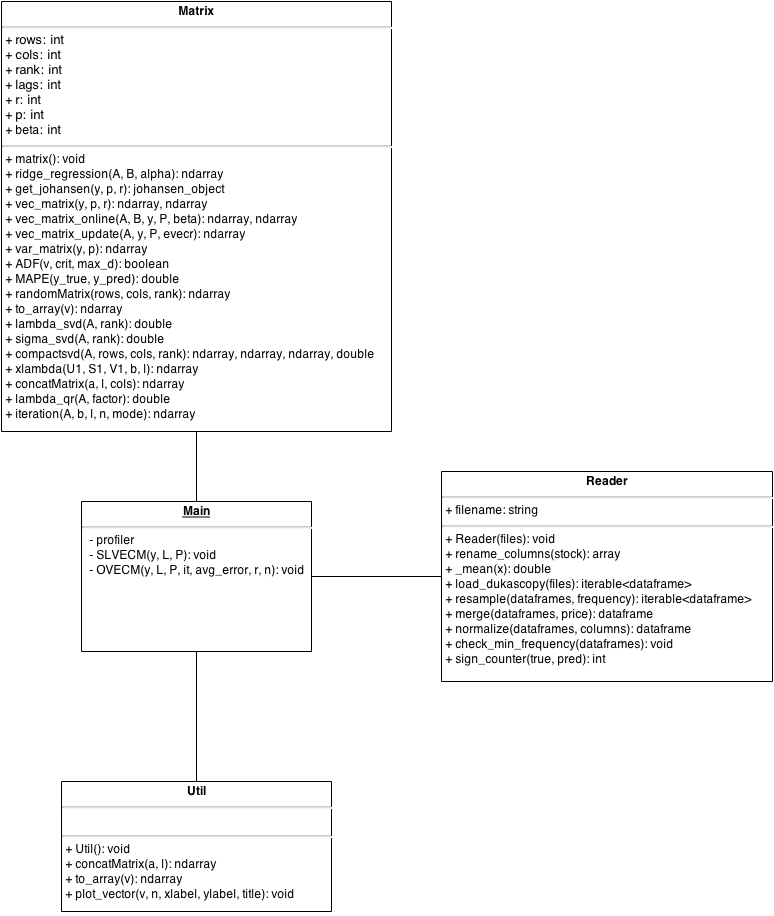
\includegraphics[width=0.8\textwidth]{images/class_diagram.png}
        \caption{Diagrama de Clases}
        \label{fig:class_diagram}
    \end{center}
\end{figure}

%\section{Métodos a paralelizar}


        \chapter{Experimentos}
        \label{ch:experimentos}
        \section{Selección de data (activos, frecuencia)}

Los datos para pruebas y experimentos se descargaron desde la plataforma
Dukascopy. Inicialmente las pruebas se realizaron con datos a frecuencia de 1
minuto, pero luego se implementó en clase Reader los métodos correspondientes
para manejar la data tick de forma automática: juntar datos de distintas
monedas (Bid o Ask), hacer un resampling a diferentes frecuencias, normalizar
las monedas dejando siempre la misma base, etc. Las divisas elegidas para
realizar los experimentos fueron: \emph{EURUSD}, \emph{GBPUSD}, \emph{USDCHF},
\emph{USDJPY} y se trabajó con el Ask Price \ref{fig:stocks_ask}. En el caso de
\emph{USDCHF}, \emph{USDJPY} se trabajó con su recíproco, para que todos los
cálculos quedaran en la misma base \emph{USD}. Además la frecuencia, muestreada
en minutos, genera una ventana de 1440 datos por día.

\begin{figure}[h!t]
    \begin{center}
        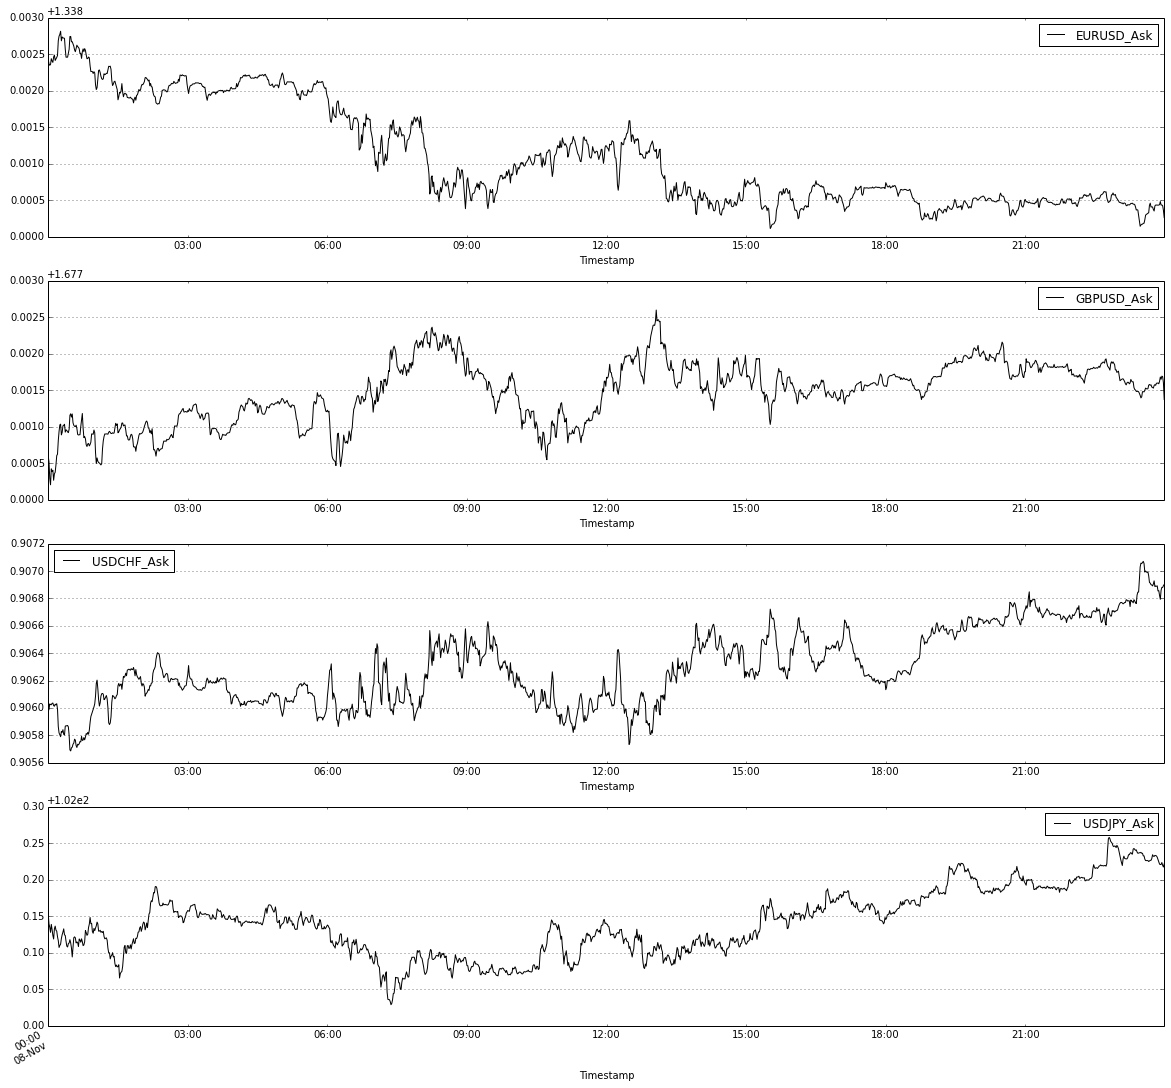
\includegraphics[width=\textwidth]{images/stocks_ask}
        \caption{Precio Ask de las divisas}
        \label{fig:stocks_ask}
    \end{center}
\end{figure}

Los ticks están compuestos por: \emph{Date}, \emph{Time}, \emph{Ask},
\emph{Bid}, \emph{AskVolume}, \emph{BidVolume}(ver tabla~\ref{tab:ticks}). Por
ser datos ticks, el campo Time es un hora \emph{double}, es decir, tiene
asociada una hora :minutos: segundos, donde segundos es un número no entero.
Cabe destacar que no existe una clara relación entre la aparición de ticks, ya
que en algunos casos aparecen hasta 4 ticks en 1 segundo, mientras que en otros
horarios no aparecen ticks en 90 segundos (dato calculado con la función
check\_min\_frequency de la clase Reader). En algunos casos, cómo en los días
más emblemáticos del año, que la cantidad de ticks por día incrementa
considerablemente, por ejemplo: un día reglar tiene aproximadamente 35 mil
ticks, mientras que días como 11 de Septiembre que hay 87 mil ticks. 

\begin{table}[h!]
\caption{Data Tick}
\label{tab:ticks}
\begin{center}
\begin{tabular}{|c|c|c|c|c|c|}
\hline
Date & Time & Ask & Bid& AskVolume & BidVolume \\
\hline
11-08-2014 & 00:00:00.000 & 1.34046 & 1.34042 & 1.25 & 1.69 \\
11-08-2014 & 00:00:02.159 & 1.34047 & 1.34043 & 4.69 & 1 \\
11-08-2014 & 00:00:02.667 & 1.34046 & 1.34042 & 1.32 & 2.44 \\
11-08-2014 & 00:00:03.175 & 1.34046 & 1.34043 & 1.32 & 1 \\
11-08-2014 & 00:00:07.058 & 1.34046 & 1.34043 & 3.75 & 1.69 \\
11-08-2014 & 00:00:07.362 & 1.34043 & 1.34041 & 2.25 & 1 \\
\hline
\end{tabular}
\end{center}
\end{table}
\newpage
En la figura \ref{fig:eurusd_ticks} se puede apreciar la data tick del EURUSD,
en una ventana de 30 minutos, donde la curva superior es la correspondiente al
Ask, y la inferior al Bid. En la figura \ref{fig:eurusd_freq} se muestra la
misma moneda pero con resamples a 1, 10, 30 y 60 segundos. El resample se
calcula con el promedio de los ticks en la ventana de 6 segundos, y para el
caso que no exista movimiento en dicho periodo, se rellena con el valor
anterior.

\begin{figure}[h!t]
    \begin{center}
        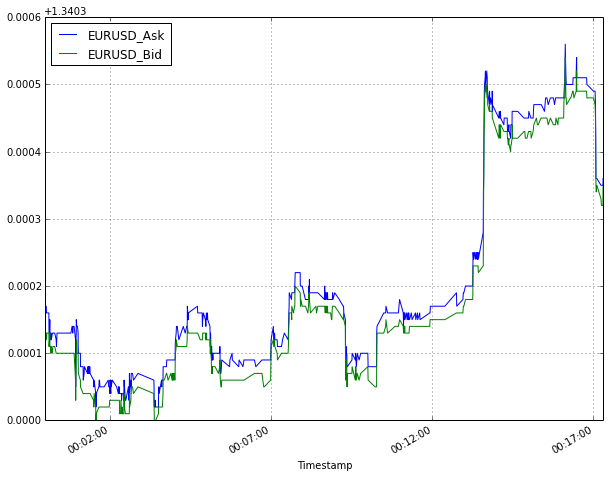
\includegraphics[width=0.7\textwidth]{images/eurusd}
        \caption{Ticks de EURUSD, Ventana de 30 minutos}
        \label{fig:eurusd_ticks}
    \end{center}
\end{figure}

\begin{figure}[h!t]
    \begin{center}
        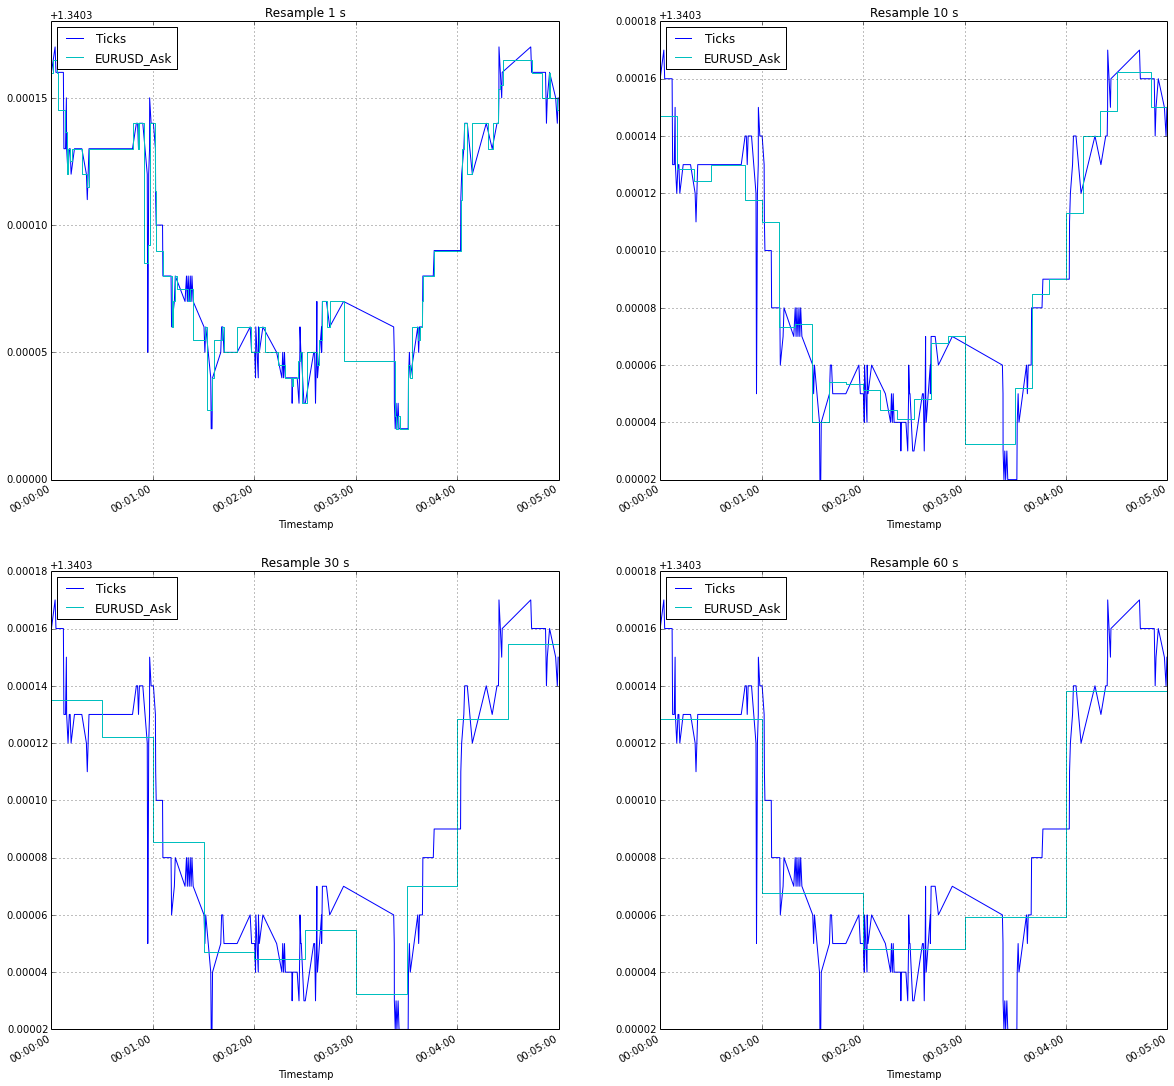
\includegraphics[width=\textwidth]{images/resample_freq}
        \caption{Ticks de EURUSD, Ventana de 30 minutos}
        \label{fig:eurusd_freq}
    \end{center}
\end{figure}

%\begin{figure}[h!t]
%    \begin{center}
%        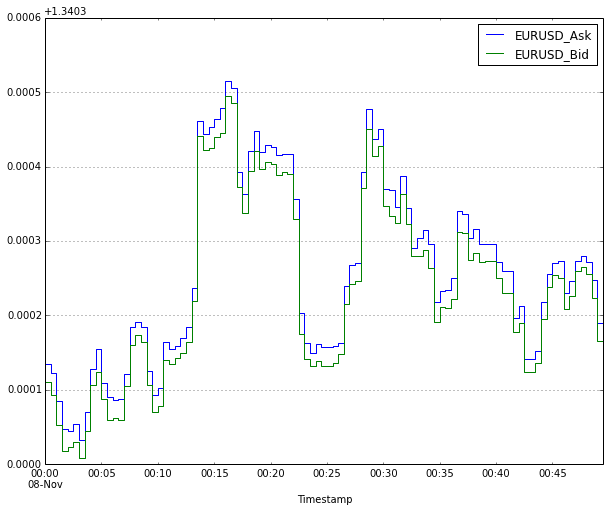
\includegraphics[width=0.6\textwidth]{images/eurusd_30s}
%        \caption{Ticks de EURUSD con resample de 30 segundos}
%        \label{fig:eurusd_30s}
%    \end{center}
%\end{figure}

\newpage
\section{Selección de Parámetros}
Cómo se mencionó anteriormente, los parámetros del algoritmo se calcularon
mediante el criterio de información de Akaike (AIC). Para esto, se tomaron
datos intra-diarios de agosto 2014, semana entre 11-15. Además, se
combinaron:
\begin{itemize}
 \item L: [100, 400, 700, 1000].
 \item P: [1, 2, 3, 4, 5].
 \item Frecuencias: 1 minuto.
\end{itemize}

Los resultados~\ref{tab:IAC} muestran para cada largo de ventana,
el número de lag óptimos (en negrita) para el modelo según el criterio de AIC.

\begin{table}[h]
\caption{Resultados de AIC}
\label{tab:IAC}
\begin{center}
\begin{tabular}{|l|c|c|c|c|c|}
\hline
\backslashbox{\textbf{L}}{\textbf{P}} & \textbf{1} & \textbf{2} & \textbf{3} & \textbf{4} & \textbf{5} \\
\hline
100 & -58.64574 & \textbf{-58.83743} & -58.70088 & -58.61984 & -58.68117 \\
400 & -60.42127 & -60.65667 & -60.67377 & -60.64634 &  \textbf{-60.68087} \\
700 & -59.05503 & -59.17413 & \textbf{-59.20871} & -59.18571 & -59.17367 \\
100 & -58.98121 & -59.09158 & \textbf{-59.12083} & -59.10099 & -59.0927 \\
\hline
\end{tabular}
\end{center}
\end{table}

\section{Pruebas de Cointegración}
Para los efectos de pruebas como se trabajó con 4 monedas, la cantidad de 
vectores de cointegración debería ser 1, 2 o 3. 

\section{Test de raíz unitaria}
Antes de correr los test, se checkearon que las series de tiempo fueran
I(1) usando el test de Augmented Dickey Fuller (ADF).

\begin{table}[h!]
\caption{Test de raíz unitaria, Frecuencia 60s}
\label{tab:adf_60s}
\begin{center}
\begin{tabular}{|l|c|c|c|c|c|}
\hline
& \textbf{Estadístico} & \textbf{Valor Crítico} & \textbf{Resultado}\\
\hline
EURUSD          & -0.64 & -1.94 & True       \\
$\Delta$ EURUSD & -70.45   & -1.94 & False       \\
GBPUSD          & -0.63   & -1.94 & True          \\
$\Delta$ GBPUSD & -54.53   & -1.94 & False       \\
CHFUSD          & -0.88   & -1.94 & True         \\
$\Delta$ CHFUSD & -98.98   & -1.94 & False       \\
JPYUSD          & -0.65 & -1.94 & True        \\
$\Delta$ JPYUSD & -85.78 & -1.94 & False     \\ 
\hline
\end{tabular}
\end{center}
\end{table}

\begin{table}[h!]
\caption{Test de raíz unitaria, Frecuencia 30s}
\label{tab:adf_30s}
\begin{center}
\begin{tabular}{|l|c|c|c|c|c|}
\hline
& \textbf{Estadístico} & \textbf{Valor Crítico} & \textbf{Resultado}\\
\hline
EURUSD          & -0.94 & -1.94 & True       \\
$\Delta$ EURUSD & -25.66   & -1.94 & False       \\
GBPUSD          & 0.29   & -1.94 & True          \\
$\Delta$ GBPUSD & -36.08   & -1.94 & False       \\
CHFUSD          & -0.49   & -1.94 & True         \\
$\Delta$ CHFUSD & -35.02   & -1.94 & False       \\
JPYUSD          & -0.45 & -1.94 & True        \\
$\Delta$ JPYUSD & -37.41 & -1.94 & False     \\ 
\hline
\end{tabular}
\end{center}
\end{table}

\begin{table}[h!]
\caption{Test de raíz unitaria, Frecuencia 10s}
\label{tab:adf_10s}
\begin{center}
\begin{tabular}{|l|c|c|c|c|c|}
\hline
& \textbf{Estadístico} & \textbf{Valor Crítico} & \textbf{Resultado}\\
\hline
EURUSD          & -0.85 & -1.94 & True       \\
$\Delta$ EURUSD & -43.91   & -1.94 & False       \\
GBPUSD          & 0.25   & -1.94 & True          \\
$\Delta$ GBPUSD & -40.81   & -1.94 & False       \\
CHFUSD          & -0.51   & -1.94 & True         \\
$\Delta$ CHFUSD & -61.12   & -1.94 & False       \\
JPYUSD          & -0.34 & -1.94 & True        \\
$\Delta$ JPYUSD & -46.38 & -1.94 & False     \\ 
\hline
\end{tabular}
\end{center}
\end{table}

Las tablas~\ref{tab:adf_60s}~\ref{tab:adf_30s}~\ref{tab:adf_60s} muestran que
todas las series no son rechazadas por el test de raíz unitaria pero si son
rechazadas para sus primeras diferencias (Con un valor crítico del 5\%). Esto
significa que todas las series de tiempo son I(1) por lo que es posible usar
los modelos VECM y OVECM. 

\section{Performance}
Dentro de todos los experimentos realizados, según la selección de parámetros
y considerando 400 iteraciones los resultados de tiempos de ejecución se pueden
ver en la tabla~\ref{tab:extimes}

\begin{table}[h!]
\caption{Tiempos de ejecución}
\label{tab:extimes}
\begin{center}
\begin{tabular}{|l|c|c|c|c|c|}
\hline
& L & P & e  & Tiempo[s] \\
\hline
OVECM & 100 &p=2  & 0      & 2.492\\
OVECM & 100 &p=2  & 0.0026  & 1.606\\
SLVECM & 100 &p=2& -- & 2.100\\
\hline
OVECM & 400 & p=5  & 0      & 3.513\\
OVECM & 400 &p=5  & 0.0041  & 2.569\\
SLVECM & 400 & p=5 & -- & 3.222\\
\hline
OVECM & 700 &p=3  & 0      & 3.296\\
OVECM & 700 &p=3  & 0.0032  & 2.856\\
SLVECM & 700 &p=3 & -- & 3.581\\
\hline
OVECM & 1000 & p=3 & 0      & 4.387\\
OVECM & 1000 & p=3  & 0.0022  & 2.408\\
SLVECM & 1000 & p=3  & -- & 3.609\\
\hline
\end{tabular}
\end{center}
\end{table}

OVECM recibe como parámetro el umbral de error para cambiar los vectores de
cointegración. Es decir, OVECM con e = 0 es lo mismo que ejecutar el SLVECM,
ambos tienen exactamente los mismos vectores de cointegración y estadísticos.

Para ver en detalle qué parte del código demora más se presenta el siguiente
profile de ejecución:
\begin{verbatim}
   Time %Time  Line Contents
============================
               def OVECM(y, L, P, it, avg_error, r, n):
      4   0.0      it2, l = y.shape
               
      7   0.0      dy_true = np.zeros([it, l], dtype=np.float32)
      4   0.0      dy_pred = np.zeros([it, l], dtype=np.float32)
      4   0.0      mape = np.zeros([it, l], dtype=np.float32)
      4   0.0      mae = np.zeros([it, l], dtype=np.float32)
      4   0.0      rmse = np.zeros([it, l], dtype=np.float32)
               
      8   0.0      m = cl.Matrix()
               
      3   0.0      start_time = time.time()
               
    911   0.0      for i in range(it):
 110712   1.6          y_i = y[i:i + L]
               
   1031   0.0          if i == 0:
                           # Initialization
   6839   0.1              beta = m.get_johansen(y_i.as_matrix(), 
                                    P, r)
  29075   0.4              A, B = m.vec_matrix(y_i, P, 
                                    beta.evecr)
                       else:
                           # Update & Out-of-sample forecast
4456245  66.1              A, B = m.vec_matrix_online(A, B, y_i, 
                                    P, beta.evecr)
   6820   0.1              dy_true[i-1, :] = B[-1,:]
  11775   0.2              dy_pred[i-1, :] = np.dot(A[-1,:], x)
               
                       # OLS
 439061   6.5          x, residuals, rank, s = np.linalg.lstsq(A, B)
  79004   1.2          Ax = np.dot(A, x)
               
                       # Internal mape
  28364   0.4          y_true = y_i.as_matrix()[-n:]
  23996   0.4          y_pred = Ax[-n:] + y_i.as_matrix()[-n - 1:-1]
               
                       # Stats info
 512572   7.6          stats = cl.stats(y_true, y_pred)
   8587   0.1          mape[i, :], mae[i,:], rmse[i,:] = stats.mape, 
                            stats.mae, stats.rmse
  36757   0.5          avg_mape = np.average(mape[i, :])
               
                       # Beta update
   2224   0.0          if avg_mape > avg_error:
 865051  12.8              beta = m.get_johansen(y_i.as_matrix(), P)
    307   0.0              r = beta.r
  41151   0.6              A = m.vec_matrix_update(A, y_i, P, 
                                beta.evecr)
  79857   1.2              x, residuals, rank, s = np.linalg.lstsq(A, B)
               
                   # model_it object
   2945   0.0      oecm = cl.model_it(y[L:L + it], dy_pred + 
                        y[L - 1:L + it - 1], dy_true, dy_pred, 
                        mape, mae, rmse)


 Time  Per Hit   % Time  Line Contents
======================================
                         @do_profile(follow=[OVECM, OVECMRR])
                         def main():
    2      2.0      0.0      path = '../data_csv/data_ticks/august_11/'
    2      2.0      0.0      assets = ['EURUSD', 'GBPUSD', 
                                    'USDCHF', 'USDJPY']
                             
    6      1.2      0.0      data_list = [path+ i +'.csv' for i in assets]
                             
    7      7.0      0.0      reader = cl.Reader(data_list)
 100M   100M.0     93.7      ticks_list = reader.load()
                         
39925  39925.0      0.0      ask_norm = reader.resample_list(ticks_list, 
                            '60s', [2, 3])            
    2      2.0      0.0      y = ask_norm
                         
    1      1.0      0.0      L = 1000
    1      1.0      0.0      P = 4
    1      1.0      0.0      it = 400
    1      1.0      0.0      r = 0
    0      0.0      0.0      n = 50
    1      1.0      0.0      avg_error = 0.002
                         
 6758K 6758K.0      6.3      oecm = OVECM(y, L, P, it, avg_error, r, n)

\end{verbatim}

Se puede observar que los cálculos más costosos son la construcción de la
matriz VECM, seguido por el cálculo de los vectores de cointegración, luego de
los estadísticos en cada paso y finalmente la resolución del sistema mediante
mínimos cuadrados. Por otro lado, el cálculo está inserto dentro de la lectura
de archivos, los cuales toman mucho más tiempo que la ejecución del algoritmo.

Cabe destacar que estos números dependen del tamaño de la ventana, número de
lags, umbral de error y cantidad de elementos para calcular el mape in-sample.

En todos los casos, ya sea incluso en frecuencias de 1 segundo, el algoritmo
OVECM, toma tiempos de ejecución menor a la frecuencia de datos, esto le
permite a un algoritmo de estrategia poder utilizar como entrada los resultados
de esta implementación.

\section{Resultados}
Uno de los objetivos del algoritmo OVECM es ser más eficiente en tiempo que el
SLVECM, pero además se busca que los errores de la extrapolación no sean tan
distintos. La tabla~\ref{tab:mapes_60s}~\ref{tab:mapes_30s}~\ref{tab:mapes_10s}
muestran los diferentes indicadores de las muestras en la interpolación
(in-sample) y la extrapolación (out-of-sample). Se puede ver que son similares,
por lo que se confirma que los vectores de cointegración se pueden mantener en
cierta medida durante el tiempo. Es importante notar además que a medida que
aumenta la frecuencia, los indicadores son menores, ya que la alta frecuencia
refleja menores fluctuaciones en los valores de las divisas.

\begin{table*}[ht!]
\caption{Métricas del modelo, Frecuencia 60s}
\label{tab:mapes_60s}
\begin{center}
\begin{adjustbox}{max width=\textwidth}
\begin{tabular}{|l|l|c|c|c|c|c|c|c|c|}
\hline
\multicolumn{4}{|c|}{Model} & \multicolumn{3}{|c|}{In-sample} &
\multicolumn{3}{|c|}{Out-of-sample} \\ 
\hline
\hline
Método & L & P & e &
MAPE & MAE& RMSE&
MAPE & MAE& RMSE \\
\hline
 OVECM  &   100  &  P=2& 0.0026  &  0.00263&  0.00085&  0.00114&  0.00309&  0.00094&  0.00131\\
 OVECM  &   400  &  P=5& 0.0041  &  0.00378&  0.00095&  0.00127&  0.00419&  0.00103&  0.00143\\
 OVECM  &   700  &  P=3& 0.0032  &  0.00323&  0.00099&  0.00130&  0.00322&  0.00097&  0.00132\\
 OVECM  &   1000 &  P=3& 0.0022  &
 \textbf{0.00175}&  \textbf{0.00062}&  \textbf{0.00087} &
 \textbf{0.00172}&  \textbf{0.00061}&  \textbf{0.00090}\\
\hline
 SLVECM  &   100 &  P=2& -  &  0.00262&  0.00085&  0.00113&  0.00310&  0.00095&  0.00132\\
 SLVECM  &   400 &  P=5& -  &  0.00375&  0.00095&  0.00126&  0.00419&  0.00103&  0.00143\\
 SLVECM  &   700 &  P=3& -  &  0.00324&  0.00099&  0.00130&  0.00322&  0.00098&  0.00132\\
 SLVECM  &   1000 &  P=3& -  &
 \textbf{0.00174}&  \textbf{0.00061}&  \textbf{0.00087}&
 \textbf{0.00172}&  \textbf{0.00061}&  \textbf{0.00090}\\
\hline
\end{tabular}
\end{adjustbox}
\end{center}
\end{table*}

\begin{table*}[ht!]
\caption{Métricas del modelo, Frecuencia 30s}
\label{tab:mapes_30s}
\begin{center}
\begin{adjustbox}{max width=\textwidth}
\begin{tabular}{|l|l|c|c|c|c|c|c|c|c|}
\hline
\multicolumn{4}{|c|}{Model} & \multicolumn{3}{|c|}{In-sample} &
\multicolumn{3}{|c|}{Out-of-sample} \\ 
\hline
\hline
Método & L & P & e &
MAPE & MAE& RMSE&
MAPE & MAE& RMSE \\
\hline
 OVECM  &   100  &  P=2 &  0.0015  &  0.00156  &  0.00056  &  0.00077  &  0.00180  &  0.00067  &  0.00095 \\
 OVECM  &   400  &  P=5 &  0.0014  &  0.00140  &  0.00050  &  0.00070  &  0.00162  &  0.00059  &  0.00085 \\
 OVECM  &   700  &  P=3 &  0.0028  &  0.00287  &  0.00078  &  0.00105  &  0.00309  &  0.00081  &  0.00112 \\
 OVECM  &   1000 &  P=3 &  0.0024  &  \textbf{0.00245}  &  \textbf{0.00058}  &  \textbf{0.00079}  &  \textbf{0.00239}
   &  \textbf{0.00057}  &  \textbf{0.00082} \\
\hline
 SLVECM  &   100 &  P=2& -  &  0.00156  &  0.00056  &  0.00077  &  0.00176  &  0.00066  &  0.00095 \\
 SLVECM  &   400 &  P=5& -  &  0.00140  &  0.00050  &  0.00069  &  0.00162  &  0.00058  &  0.00085 \\
 SLVECM  &   700 &  P=3& -  &  0.00287  &  0.00077  &  0.00105  &  0.00308  &  0.00081  &  0.00111 \\
 SLVECM  &   1000&  P=3& -  &  \textbf{0.00245}  &  \textbf{0.00058}  &  \textbf{0.00079}  &  
  \textbf{0.00239}  &  \textbf{0.00057}  &  \textbf{0.00082} \\
\hline
\end{tabular}
\end{adjustbox}
\end{center}
\end{table*}

\begin{table*}[ht!]
\caption{Métricas del modelo, Frecuencia 10s}
\label{tab:mapes_10s}
\begin{center}
\begin{adjustbox}{max width=\textwidth}
\begin{tabular}{|l|l|c|c|c|c|c|c|c|c|}
\hline
\multicolumn{4}{|c|}{Model} & \multicolumn{3}{|c|}{In-sample} &
\multicolumn{3}{|c|}{Out-of-sample} \\ 
\hline
\hline
Método & L & P & e &
MAPE & MAE& RMSE&
MAPE & MAE& RMSE \\
\hline
 OVECM  &   100  &  P=2 &  0.0012  &  0.00124  &  0.00047  &  0.00065  &  0.00135  &  0.00052  &  0.00073 \\
 OVECM  &   400  &  P=5 &  0.0010  &  0.00108  &  0.00043  &  0.00061  &  0.00113  &  0.00047  &  0.00067 \\
 OVECM  &   700  &  P=3 &  0.0008  &  0.00085  &  0.00031  &  0.00045  &  0.00086  &  0.00032  &  0.00048 \\
 OVECM  &   1000 &  P=3 &  \textbf{0.0062}  &  \textbf{0.00062}  &  \textbf{0.00020}  &  \textbf{0.00033}  &  
      \textbf{0.00062}  &  \textbf{0.00020}  &  \textbf{0.00033} \\
\hline
 SLVECM  &   100 &  P=2 & -  &  0.00124  &  0.00047  &  0.00065  &  0.00136  &  0.00052  &  0.00073 \\
 SLVECM  &   400 &  P=5 & -  &  0.00108  &  0.00043  &  0.00061  &  0.00113  &  0.00047  &  0.00067 \\
 SLVECM  &   700 &  P=3 & -  &  0.00084  &  0.00031  &  0.00045  &  0.00086  &  0.00032  &  0.00048 \\
 SLVECM  &   1000 &  P=3& -  &  \textbf{0.00063}  &  \textbf{0.00020}  &  \textbf{0.00033}  &  
      \textbf{0.00063}  &  \textbf{0.00020}  &  \textbf{0.00033} \\
\hline
\end{tabular}
\end{adjustbox}
\end{center}
\end{table*}

En la figura~\ref{fig:accuracy} se puede observar qué tan bien aproxima el
método OVECM para cada divisa. En la figura~\ref{fig:mapes} se puede observar
cuánto es el error de aproximación medido en MAPE para cada iteración.

\begin{figure}[h!t]
    \begin{center}
        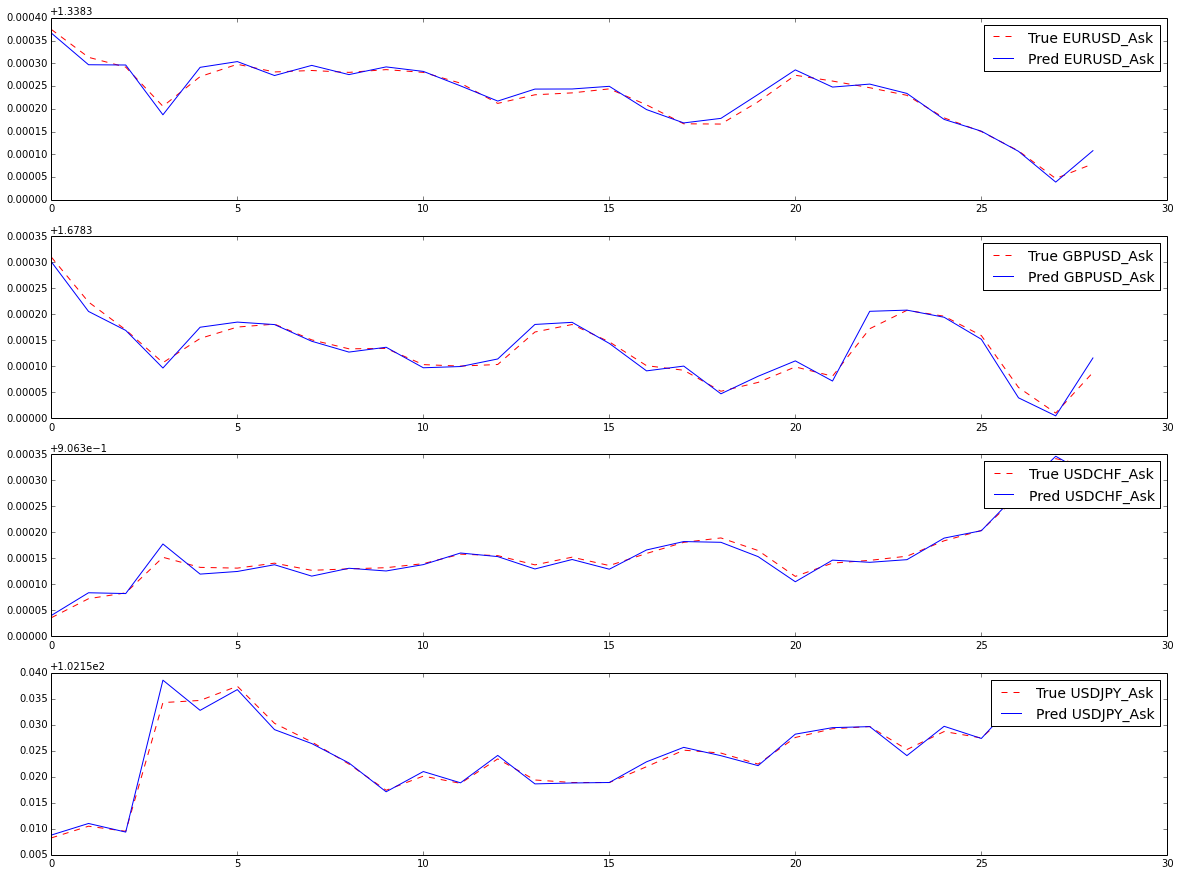
\includegraphics[width=\textwidth]{images/y_vs_yhat}
        \caption{Divisas: Valor real y aproximación}
        \label{fig:accuracy}
    \end{center}
\end{figure}


\begin{figure}[h!t]
    \begin{center}
        %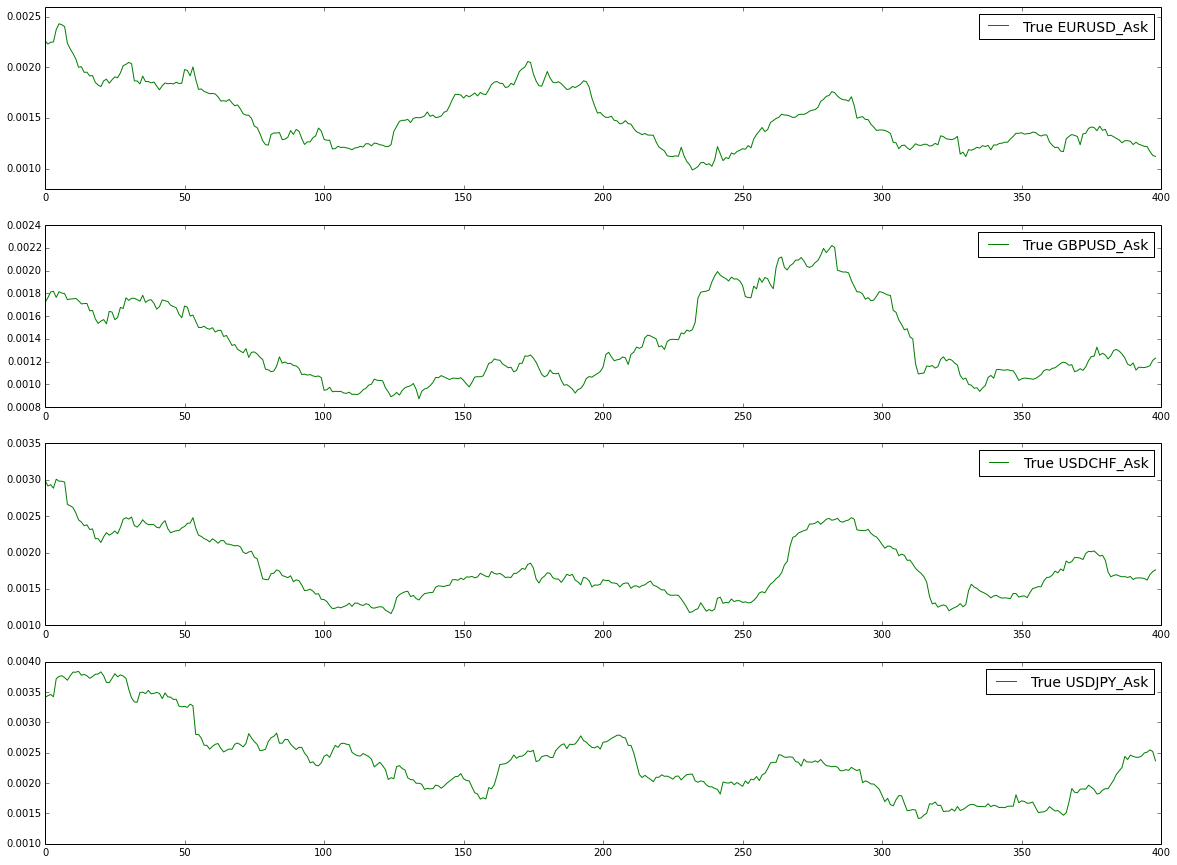
\includegraphics[width=\textwidth]{images/ovecm_mapes}
        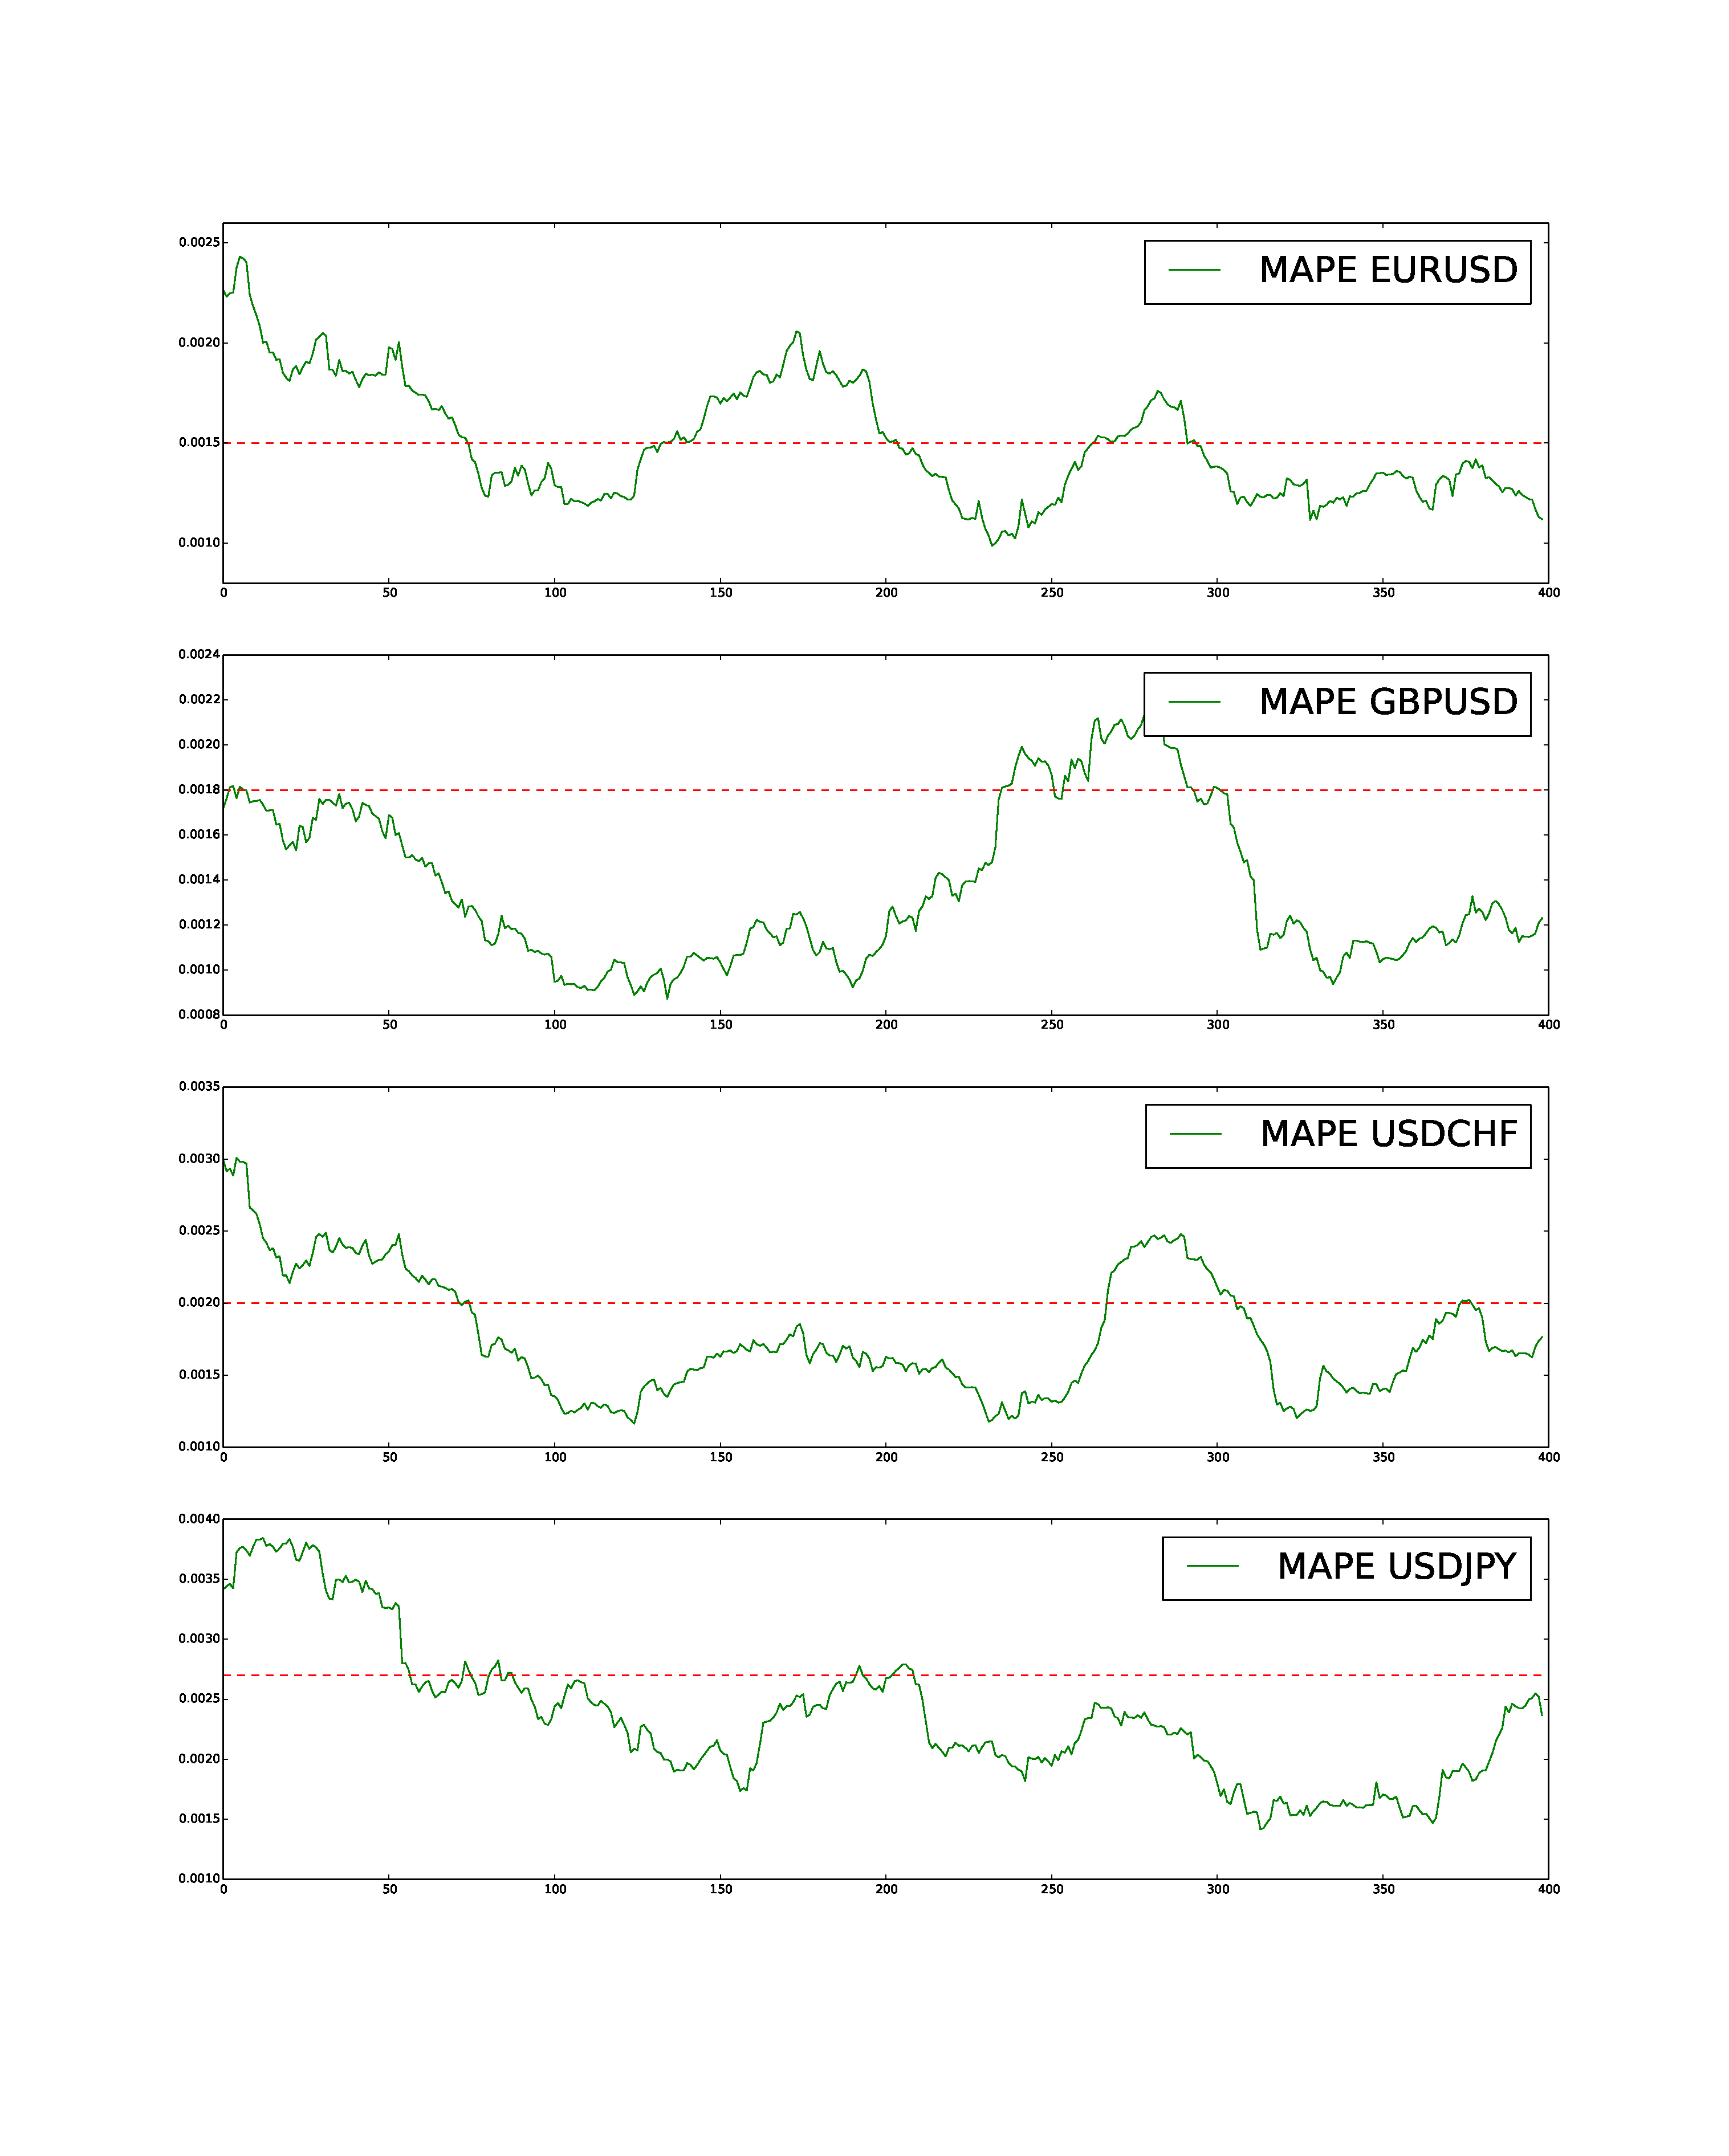
\includegraphics[width=\textwidth]{images/mapes}
        \caption{Divisas: Valor del MAPE en cada iteración}
        \label{fig:mapes}
    \end{center}
\end{figure}


	%TODO
        \chapter{Conclusiones}
        \label{ch:conclusiones}
        Lorem ipsum dolor sit amet, consectetur adipiscing elit. Aenean eget tellus
dignissim, porta leo id, placerat est. Nam a libero nec arcu hendrerit pharetra
at a mi. Donec sagittis quis est id tempor. Maecenas imperdiet, mi at
sollicitudin faucibus, tellus turpis auctor lorem, ac lacinia magna tortor sit
amet neque. Ut iaculis sit amet purus sed consequat. Nunc pretium est non erat
lacinia faucibus. Phasellus id rutrum mi. Morbi nunc nisi, mattis sit amet
purus eget, convallis tristique urna. Curabitur quis tellus placerat, eleifend
nisi eget, scelerisque quam. Nulla et sapien fermentum, dictum elit non,
elementum elit.

Morbi pretium dolor vel vestibulum pulvinar. Donec lobortis arcu malesuada
augue dictum, et pulvinar lectus viverra. Praesent rhoncus, sapien sed
porttitor volutpat, nisi ex mattis massa, tincidunt accumsan sapien sem et
elit. Maecenas sed sem accumsan, sollicitudin nunc quis, imperdiet lectus.
Maecenas ut arcu vitae odio suscipit sollicitudin. Pellentesque sed est lacus.
Quisque nec lorem sem. Nulla tristique tempus lacus, ornare maximus magna
interdum non. Proin aliquet quis ligula eget condimentum. Phasellus egestas in
libero posuere dapibus. Sed vestibulum ullamcorper arcu, eu tempus lacus
ultrices at. Ut id commodo erat, tincidunt suscipit mi. Donec suscipit lacus
sed ex molestie, nec dignissim nunc volutpat. Cras a mollis tortor, a egestas
enim. Vestibulum rhoncus orci eget purus volutpat, non viverra justo porttitor.

Ut a nulla tortor. Nam urna tortor, accumsan eu est a, rutrum ornare lectus.
Nam vestibulum libero sed consectetur vehicula. Sed non neque nec velit sodales
feugiat consequat eu tellus. Sed ut elit rutrum ipsum tristique tempus.
Phasellus sit amet porta dolor. Fusce sodales bibendum tellus vel ultrices.
Integer vitae laoreet eros.


        \addcontentsline{toc}{chapter}{\bibname}
        \bibliographystyle{apalike}
        %\bibliographystyle{plain}
        \bibliography{references}
        \nocite{*}
    \end{spacing}
\end{document}

